\chapter{Introduction to Modern Cosmology}
\label{ch:introduction}

This course explores modern cosmology from its theoretical foundations to the observational techniques that have transformed it into a precision science. We will develop the mathematical framework of general-relativistic cosmology, study the physics of the cosmic microwave background and large-scale structure, and connect these to real observational data through computational exercises. The emphasis throughout is on building physical intuition alongside quantitative rigour, and on understanding how theory and observation constrain one another.

% ===================================================================
\section{What is Cosmology?}
\label{sec:what_is_cosmology}
% ===================================================================

Cosmology addresses the oldest and most fundamental questions in science:
\begin{itemize}
    \item How did the Universe begin? Did it even have a beginning?
    \item What physical laws govern the evolution of the Universe on the largest scales?
    \item What is the ultimate fate of the Universe?
\end{itemize}
At its core, cosmology is the study of the Universe as a whole---its origin, structure, evolution, and eventual destiny. Unlike most branches of physics, we have only one Universe to observe, and we can never step outside it. This makes cosmology a uniquely constrained endeavour, yet one that has made extraordinary progress over the past century.

\subsection{The Cosmological Principle}

Any scientific theory of the Universe must start from a simplifying assumption, since without one the problem is hopelessly complex. The foundational assumption of modern cosmology is the \textbf{Cosmological Principle}: \textit{viewed on sufficiently large scales, the Universe is homogeneous and isotropic}. Homogeneity means that the statistical properties of the Universe are the same at every point; isotropy means they are the same in every direction.

The cosmological principle can be understood as an extension of the Copernican principle---the philosophical stance that there are no privileged observers. Applied to cosmology, this means that the Universe should look broadly the same to any observer, regardless of their location. It was first articulated in a cosmological context by Isaac Newton in the \textit{Philosophi\ae{} Naturalis Principia Mathematica} (1687), though its modern formulation is due to the work of Einstein, Friedmann, Lema\^{i}tre, Robertson, and Walker in the early twentieth century.

Of course, the Universe is manifestly \emph{not} homogeneous on small scales: stars, galaxies, clusters, filaments, and voids represent enormous density contrasts. The cosmological principle applies only on scales larger than roughly $100$--$200\,\mathrm{Mpc}$, above which galaxy surveys confirm that the distribution of matter becomes statistically uniform.

\subsection{Olbers' Paradox}
\label{sec:olbers}

A simple but profound consequence of taking the cosmological principle seriously is \textbf{Olbers' paradox}, posed by Heinrich Olbers in 1823 (though considered earlier by Thomas Digges in 1576 and others): \textit{why is the night sky dark?}

If the Universe were infinite in spatial extent, infinite in age, static, and uniformly populated with luminous stars, then every line of sight would eventually terminate on the surface of a star. We can make this quantitative. Stars are luminous spheres with typical radii $R_{\star}\sim\Rsun\sim 7\times 10^{8}\,\mathrm{m}\sim 2\times 10^{-14}\,\mathrm{Mpc}$, and the number density of stars in the Universe is roughly $n_{\star}\sim 10^{9}\,\mathrm{Mpc}^{-3}$. The mean free path before a line of sight intercepts a stellar disc is
\begin{equation}
\boxed{\lambda = \frac{1}{n_{\star}\,\pi R_{\star}^2} \sim \frac{1}{(10^{9}\,\mathrm{Mpc}^{-3})(10^{-27}\,\mathrm{Mpc}^2)} \sim 10^{18}\,\mathrm{Mpc}\,.}
\label{eq:olbers_mfp}
\end{equation}
In an infinite, static, eternal universe every sightline would eventually hit a star, and the entire sky would glow with the surface brightness of a typical stellar photosphere.

Several resolutions have been proposed:
\begin{enumerate}
    \item \textbf{Absorption by intervening material.} Dust or gas could block the light from distant stars. However, in a universe of infinite age, the absorbing material would itself reach thermal equilibrium with the radiation field and re-radiate at the same temperature. This does not resolve the paradox in the long run.
    \item \textbf{The Universe has finite spatial extent} (or stars occupy only a finite volume), so that $r \ll 10^{18}\,\mathrm{Mpc}$.
    \item \textbf{The Universe has a finite age} (or stars have a finite age), so that $ct \ll 10^{18}\,\mathrm{Mpc}$. Light from stars beyond the horizon $ct$ has not yet had time to reach us.
    \item \textbf{Cosmic expansion reduces the surface brightness of distant sources} through redshift, which shifts photons to longer wavelengths and dilutes their arrival rate.
\end{enumerate}
The primary resolution is~(3): the Universe has a finite age of approximately $13.8\,\mathrm{Gyr}$, corresponding to a comoving horizon of order $10^{4}\,\mathrm{Mpc}$---far smaller than $\lambda$. The expansion of the Universe (resolution~4) contributes an additional, though secondary, dimming effect.

\subsection{Units in Cosmology}

Throughout these notes we adopt the standard units of extragalactic astronomy and cosmology:
\begin{itemize}
    \item \textbf{Time:} $1\,\mathrm{Gyr} = 10^{9}\,\mathrm{yr} \approx 3.2\times 10^{16}\,\mathrm{s}$.
    \item \textbf{Distance:} $1\,\mathrm{Mpc} = 10^{6}\,\mathrm{pc} \approx 3.1\times 10^{22}\,\mathrm{m}$.
    \item \textbf{Mass:} $1\,\Msun \approx 2\times 10^{30}\,\mathrm{kg}$.
\end{itemize}
The speed of light is $c\approx 3\times 10^{8}\,\mathrm{m\,s^{-1}}$, and Newton's gravitational constant is $G\approx 6.67\times 10^{-11}\,\mathrm{m^3\,kg^{-1}\,s^{-2}}$.


% ===================================================================
\section{A Brief History of Cosmology}
\label{sec:history}
% ===================================================================

\subsection*{The Great Debate and the Discovery of External Galaxies}

It could be argued that the field of cosmology began in earnest when we determined that some objects lie outside our own Galaxy. In 1920, Harlow Shapley (Mount Wilson Observatory) and Heber Curtis (Lick Observatory) engaged in what is now known as ``The Great Debate.'' Shapley argued that the Universe comprised a single large galaxy, while Curtis maintained that the observed spiral nebulae were ``island universes''---independent stellar systems far beyond the Milky Way.

Evidence soon mounted in favour of Curtis's view. In 1922, John Charles Duncan discovered variable stars in M33 (the Triangulum Galaxy). In 1924, Knut Lundmark estimated distances to spiral nebulae using galaxy diameters, though his non-standard method was largely ignored at the time. The decisive breakthrough came in 1924 when Edwin Hubble identified Cepheid variable stars in the Andromeda Nebula (M31) and M33, calibrating their distances through the well-established Cepheid period--luminosity relation and proving conclusively that these nebulae were far too distant to be part of the Milky Way.

\subsection*{Redshift}

A key observable in cosmology is the \textbf{redshift} of spectral lines. If a spectral line has rest-frame (emitted) wavelength $\lambda_{\mathrm{e}}$ and is observed at wavelength $\lambda_{\mathrm{o}}$, the redshift is defined as
\begin{equation}
\boxed{z \equiv \frac{\lambda_{\mathrm{o}} - \lambda_{\mathrm{e}}}{\lambda_{\mathrm{e}}}\,.}
\label{eq:redshift_intro}
\end{equation}
A positive $z$ corresponds to a shift toward longer (redder) wavelengths. As we shall see, this cosmological redshift arises not from a Doppler effect due to the motion of galaxies through space, but from the stretching of space itself during the photon's journey.

\subsection{Hubble's Law and the Expanding Universe}

In 1929, Edwin Hubble combined redshift measurements for nearly 50 galaxies with distance estimates for about 20 of them to discover a striking linear relationship between a galaxy's recession velocity and its distance:
\begin{equation}
\boxed{v = \Hnot\, d\,,}
\label{eq:hubble_law}
\end{equation}
now known as \textbf{Hubble's law}. Hubble's original analysis yielded $\Hnot = 500\kmsMpc$, a value that was far too large because he had severely underestimated the distances to galaxies.

%\begin{figure}[H]
%\centeringa
% TODO: Add figure --- Hubble's 1929 velocity--distance diagram
%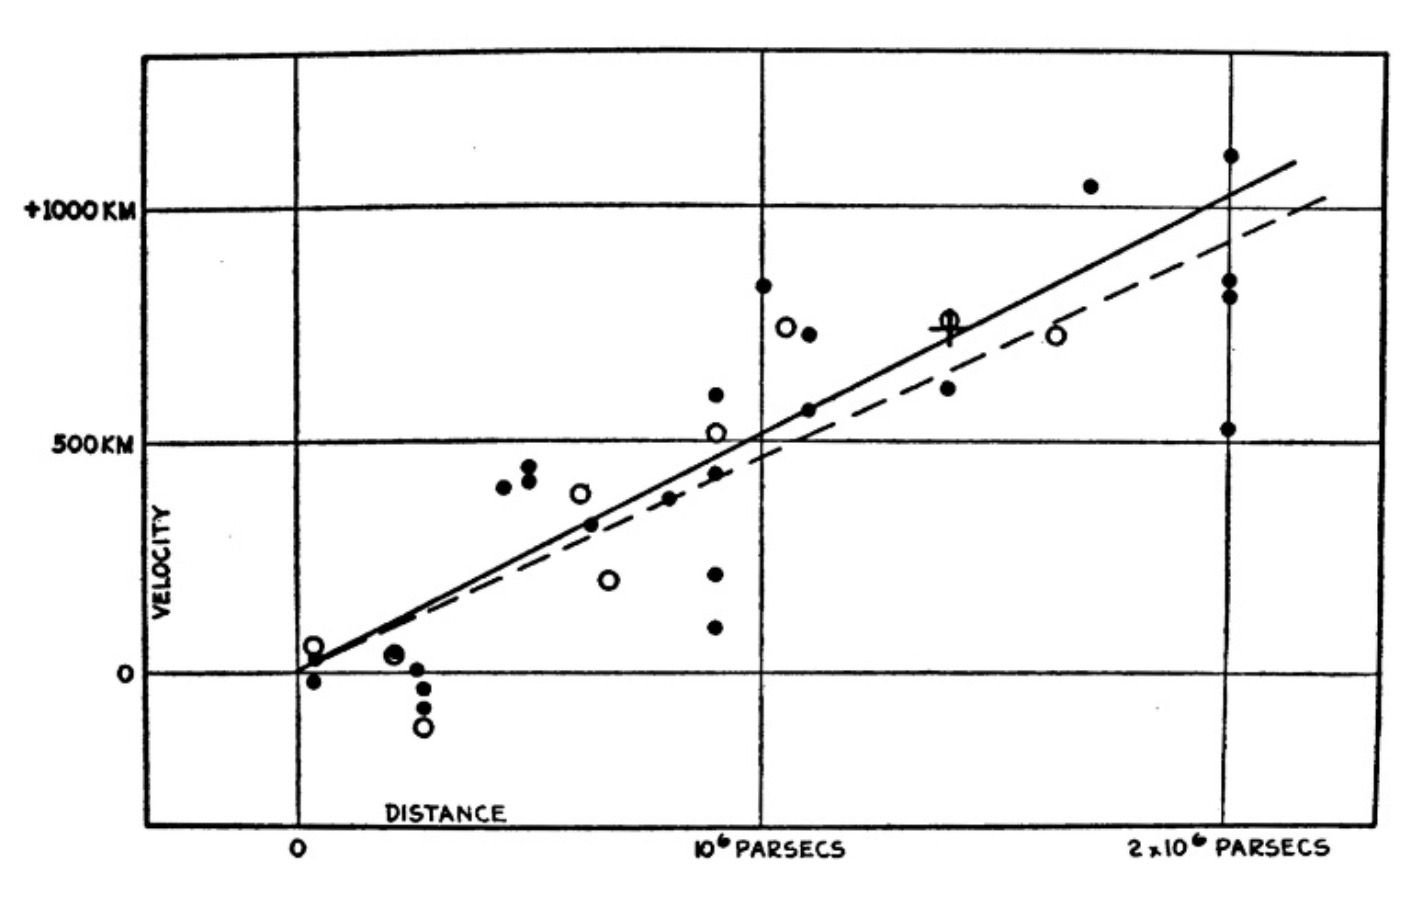
\includegraphics[width=0.9\columnwidth]{figures/hubble_original.png}
%\fbox{\parbox{0.8\textwidth}{\centering\vspace{2cm}\textit{Figure placeholder: Hubble's 1929 original velocity--distance diagram}\vspace{2cm}}}
%\caption{Hubble's 1929 velocity--distance diagram for nearby galaxies, providing the first observational evidence for a linear relation between recession velocity and distance.}
%\label{fig:hubble_1929}
%\end{figure}

As with many cases in science, the discovery was not named after its original discoverer. Two years before Hubble, in 1927, the Belgian Catholic priest, mathematician and astronomer Georges Lema\^{i}tre independently derived the velocity--distance relation from solutions of Einstein's field equations and estimated the proportionality constant from available data. The International Astronomical Union (IAU) now recommends the name \textbf{Hubble--Lema\^{i}tre law} in recognition of Lema\^{i}tre's contribution.

%\begin{figure}[H]
%\centering
% TODO: Add figure --- Lematre 1927 and Hubble 1929 diagrams side by side
%\fbox{\parbox{0.8\textwidth}{\centering\vspace{2cm}\textit{Figure placeholder: Lema\^{i}tre (1927) and Hubble (1929) diagrams side by side}\vspace{2cm}}}
%\caption{Left: Lema\^{i}tre's 1927 velocity--distance relation. Right: Hubble's 1929 version of the same relation. Both point to the same conclusion---the Universe is expanding.}
%\label{fig:lemaitre_hubble}
%\end{figure}

Seventy years of subsequent work dramatically refined the measurement. In 2001, Wendy Freedman and collaborators used the Hubble Space Telescope Key Project to calibrate distances to nearby galaxies and found $\Hnot = 70 \pm 7\kmsMpc$, consistent with the modern best estimates.

\begin{figure}[H]
\centering
% TODO: Add figure --- Freedman et al. (2001) Hubble diagram
%\fbox{\parbox{0.8\textwidth}{\centering\vspace{2cm}\textit{Figure placeholder: Freedman et al.\ (2001) HST Key Project Hubble diagram}\vspace{2cm}}}
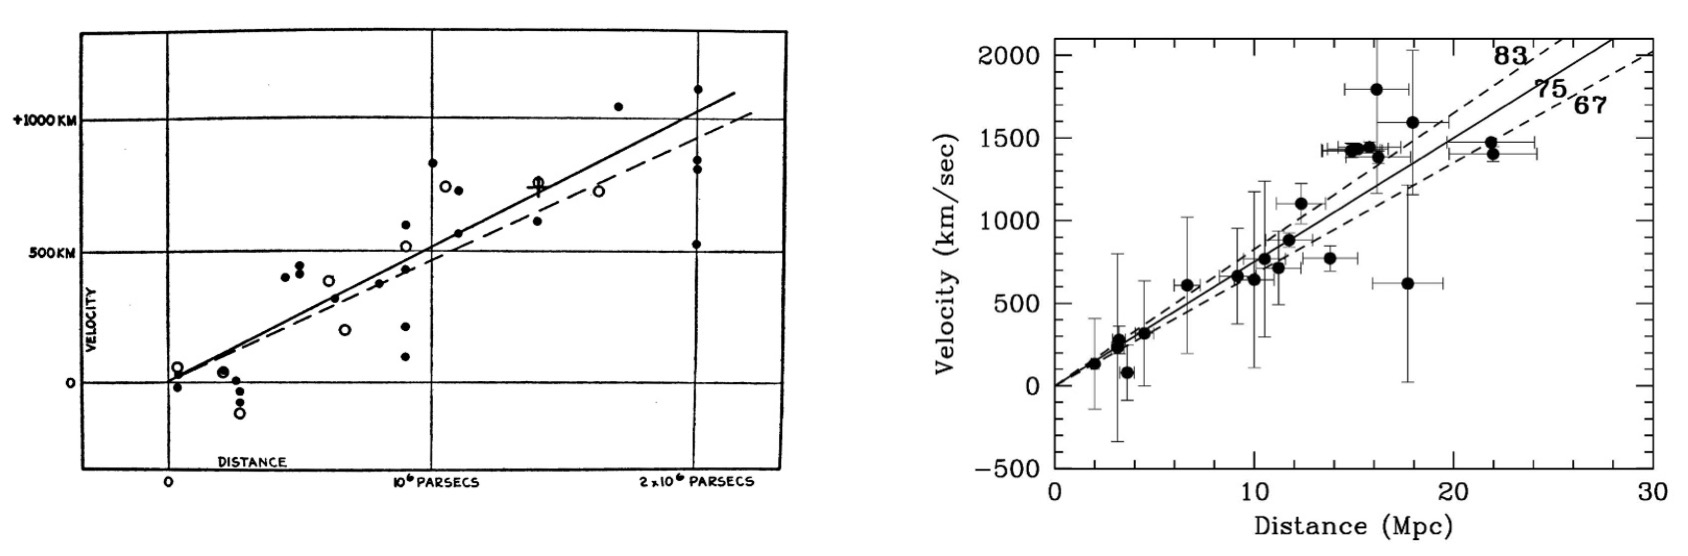
\includegraphics[width=0.9\columnwidth]{figures/hubble_modern.png}
\caption{{\em Left: } Hubble's 1929 velocity--distance diagram for nearby galaxies, providing the first observational evidence for a linear relation between recession velocity and distance. {\em Right:} The Hubble diagram from the HST Key Project (Freedman et al.\ 2001), yielding $\Hnot = 70 \pm 7\kmsMpc$ from multiple distance indicators.}
\label{fig:freedman_2001}
\end{figure}


% ===================================================================
\section{The Scale Factor and Homogeneous Expansion}
\label{sec:scale_factor}
% ===================================================================

Hubble's law tells us that galaxies are receding from us with velocities proportional to their distance. At first glance, this seems to place us at the centre of the Universe, violating the cosmological principle. The resolution is that the expansion is \emph{homogeneous and isotropic}: every observer, regardless of their location, sees the same Hubble law.

\subsection*{The Triangle Argument}

To see this concretely, consider three galaxies at positions $\vec{r}_1$, $\vec{r}_2$, and $\vec{r}_3$. The sides of the triangle they form are
\begin{equation}
    r_{12} = |\vec{r}_1 - \vec{r}_2|, \qquad r_{23} = |\vec{r}_2 - \vec{r}_3|, \qquad r_{31} = |\vec{r}_3 - \vec{r}_1|\,.
\end{equation}
A homogeneous and isotropic expansion must preserve the shape of this triangle---that is, the ratios of the side lengths must remain constant. The only expansion law compatible with this requirement is
\begin{equation}
    r_{12}(t) = a(t)\,r_{12}(t_0), \qquad r_{23}(t) = a(t)\,r_{23}(t_0), \qquad r_{31}(t) = a(t)\,r_{31}(t_0),
\label{eq:scale_factor_triangle}
\end{equation}
where $a(t)$ is a universal function of time called the \textbf{scale factor}, normalised so that $a(t_0) = 1$ at the present epoch~$t_0$. The scale factor is independent of both position and direction---it encodes the entire expansion history of the Universe.

\begin{figure}[H]
\centering
% TODO: Add figure --- Homogeneous expansion triangle / balloon analogy
%\fbox{\parbox{0.8\textwidth}{\centering\vspace{2cm}\textit{Figure placeholder: Homogeneous expansion of a triangle of galaxies}\vspace{2cm}}}
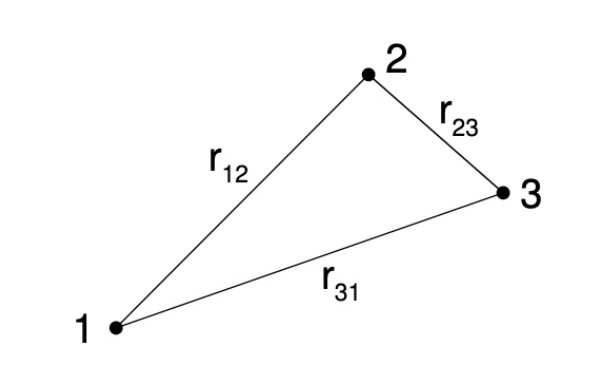
\includegraphics[width=0.6\columnwidth]{figures/triangle.png}
\caption{Illustration of homogeneous expansion: a triangle of galaxies at two different times. All inter-galaxy distances are rescaled by the same factor $a(t)$, preserving the shape of the triangle.}
\label{fig:expansion_triangle}
\end{figure}

\subsection*{Deriving Hubble's Law from the Scale Factor}

At any time $t$, an observer in galaxy~1 sees galaxy~2 receding with velocity
\begin{equation}
    v_{12}(t) = \frac{\dd r_{12}}{\dd t} = \dot{a}(t)\,r_{12}(t_0) = \frac{\dot{a}}{a}\,r_{12}(t)\,.
\end{equation}
The same applies to any pair of galaxies. Defining the \textbf{Hubble parameter}
\begin{equation}
\boxed{H(t) \equiv \frac{\dot{a}(t)}{a(t)}\,,}
\label{eq:hubble_parameter}
\end{equation}
we recover the general form of Hubble's law: $v = H(t)\,r$. Evaluated at the present time, $H(t_0) \equiv \Hnot$ is the \textbf{Hubble constant}. Crucially, an observer in any galaxy derives exactly the same Hubble law with the same value of~$H$, consistent with the cosmological principle.

\subsection*{General Relativity and the Friedmann Equations}

The mathematical framework that underpins the expanding universe is Einstein's General Theory of Relativity (1915), which describes gravity not as a force but as the curvature of spacetime caused by the presence of mass and energy. In 1917, Willem de Sitter found both static and expanding solutions to Einstein's field equations, though Einstein and de Sitter initially preferred the static case. In 1922, Alexander Friedmann derived the general non-static solutions describing universes that can expand or contract---pointing out an error in Einstein's earlier analysis. We will derive these \textit{Friedmann equations} in full detail in Chapter~\ref{ch:background_dynamics}.


% ===================================================================
\section{Big Bang vs.\ Steady State}
\label{sec:bb_vs_ss}
% ===================================================================

Hubble's discovery of the expanding Universe was a major advance, but it did not immediately settle the question of the Universe's origin. Two competing models emerged:

\begin{itemize}
    \item \textbf{The Hot Big Bang Model} (Hubble, Lema\^{i}tre): The Universe began in an extremely hot, dense state and has been expanding and cooling ever since. The cosmological principle holds, but the Universe evolves with time---its temperature, density, and composition all change.
    \item \textbf{The Steady State Model} (Bondi, Gold, and Hoyle, 1948): The Universe obeys a ``perfect cosmological principle''---it is homogeneous and isotropic not only in space but also in time. Although it expands, matter is continuously created to maintain a constant average density.
\end{itemize}

\begin{figure}[H]
\centering
% TODO: Add figure --- Big Bang vs Steady State schematic
%\fbox{\parbox{0.8\textwidth}{\centering\vspace{2cm}\textit{Figure placeholder: Schematic comparison of the Hot Big Bang and Steady State models}\vspace{2cm}}}
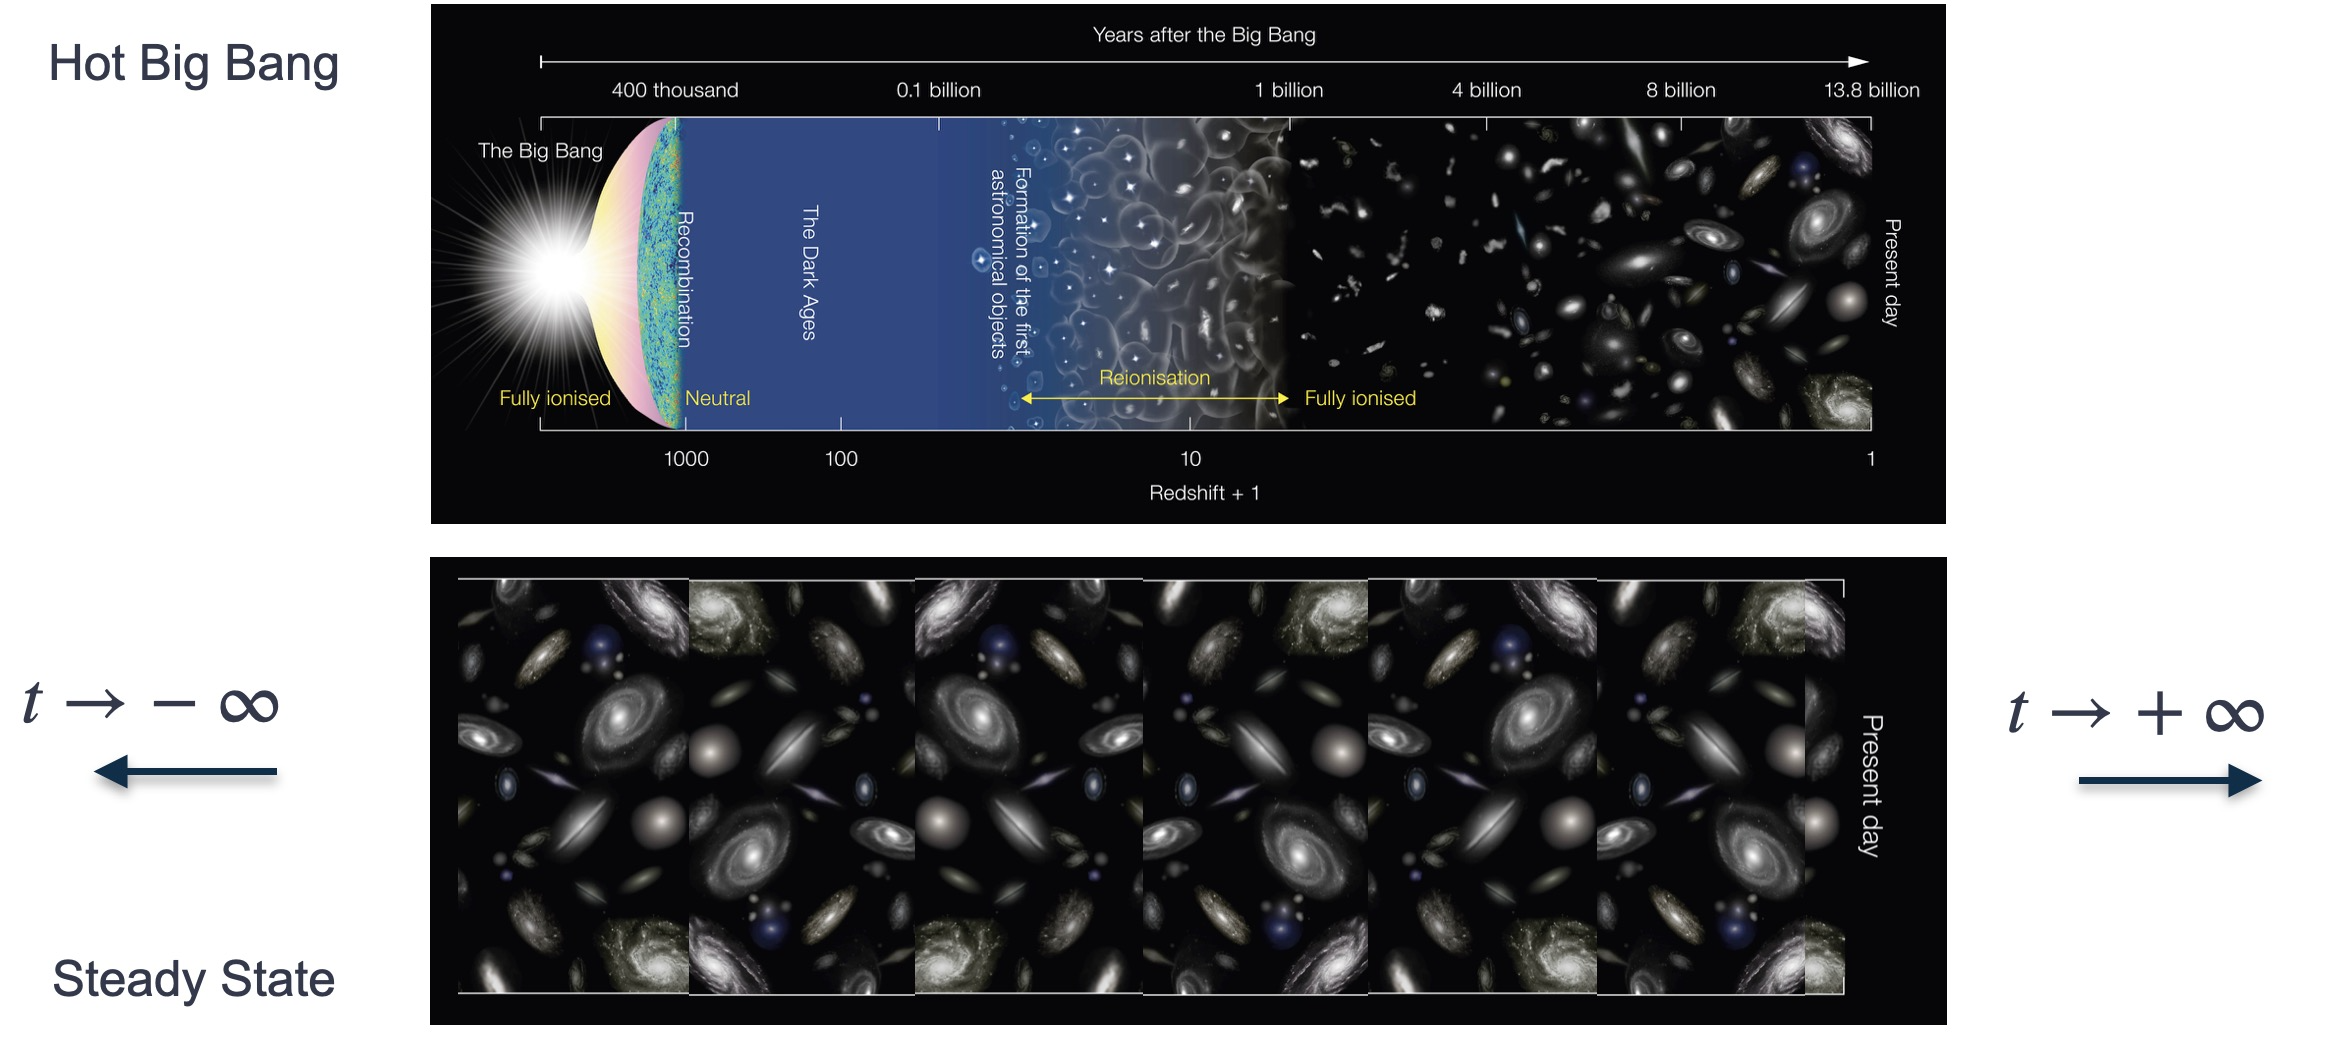
\includegraphics[width=\columnwidth]{figures/big_bang_steady_state.png}
\caption{Schematic comparison of the Hot Big Bang and Steady State models. In the Big Bang model, the Universe has a finite age and evolves from an initial singularity. In the Steady State model, the Universe has existed forever in roughly the same state, with continuous matter creation compensating for the dilution due to expansion.}
\label{fig:bb_vs_ss}
\end{figure}

Through the 1950s and 1960s, the ``Great Debate'' shifted to the question of which model correctly described our Universe. Several observations ultimately ruled out the Steady State model:
\begin{enumerate}
    \item \textbf{Quasar evolution} (M.~Schmidt 1963; M.~Rees and D.~Sciama 1965): The abundance of quasars (quasi-stellar objects) at high redshift is much larger than at low redshift, violating the time symmetry required by the perfect cosmological principle.
    \item \textbf{The Cosmic Microwave Background} (A.~Penzias and R.~Wilson 1965): The discovery of a pervasive thermal radiation field at $T\approx 3\,\mathrm{K}$, naturally explained as the cooled remnant of the hot early Universe, had no satisfactory explanation in the Steady State framework.
    \item \textbf{Singularity theorems} (S.~Hawking and G.~Ellis 1966): On purely theoretical grounds, Hawking showed that any plausible general-relativistic cosmology satisfying reasonable energy conditions must contain an initial singularity, undermining the premise of an eternal, unchanging Universe.
\end{enumerate}

Together, these observations and theoretical results firmly established the Hot Big Bang as the standard model of cosmology.


% ===================================================================
\section{Discovery of the Cosmic Microwave Background}
\label{sec:cmb_discovery}
% ===================================================================

The discovery of the cosmic microwave background (CMB) radiation is one of the most important events in the history of cosmology, providing direct evidence for the hot, dense early Universe predicted by the Big Bang model.

\subsection*{Penzias and Wilson (1965)}

In 1965, Arno Penzias and Robert Wilson, working at Bell Telephone Laboratories in Holmdel, New Jersey, were using a sensitive horn antenna---originally built for satellite communications---to survey the sky at microwave frequencies. They cooled the receiver with liquid helium to suppress thermal noise from the detector itself. Despite meticulous elimination of all known sources of interference (including removing what they diplomatically described as a ``white dielectric material'' deposited by pigeons nesting in the antenna), they found a persistent, isotropic background signal corresponding to an antenna temperature of approximately $3.5\,\mathrm{K}$ at a wavelength of $7.35\,\mathrm{cm}$.

At the same time and by coincidence, Jim Peebles at Princeton University had independently predicted the existence of a cosmic background radiation as a relic of the hot early Universe. When Penzias contacted the Princeton group, Robert Dicke, Peter Roll, and David Wilkinson visited Bell Labs to examine the data and the experimental setup. Once convinced of the result, the two groups published companion papers in the \textit{Astrophysical Journal} (volume 142):
\begin{itemize}
    \item Dicke, Peebles, Roll \& Wilkinson: ``Cosmic Black-Body Radiation'' (theoretical interpretation).
    \item Penzias \& Wilson: ``A Measurement of Excess Antenna Temperature at 4080~Mc/s'' (observational detection).
\end{itemize}
Penzias and Wilson were awarded the Nobel Prize in Physics in 1978 for this discovery.

%\begin{figure}[H]
%\centering
% TODO: Add figure --- Penzias and Wilson with the horn antenna
%\fbox{\parbox{0.8\textwidth}{\centering\vspace{2cm}\textit{Figure placeholder: Penzias and Wilson with the Bell Labs horn antenna}\vspace{2cm}}}
%\caption{Arno Penzias and Robert Wilson standing in front of the horn antenna at Bell Telephone Laboratories, Holmdel, New Jersey, with which they discovered the cosmic microwave background radiation in 1965.}
%\label{fig:penzias_wilson}
%\end{figure}

Remarkably, the CMB may have been observed even earlier. In 1940, Andrew McKellar detected excited rotational states of cyanogen (CN) molecules in interstellar space, corresponding to an excitation temperature of approximately $2.3\,\mathrm{K}$. Walter Adams confirmed similar observations in 1941. These measurements were not, however, interpreted as evidence for a cosmic radiation background at the time.

\subsection*{The Search for Anisotropies}

If the large-scale structure we observe today---galaxies, clusters, voids, and filaments---grew from small initial fluctuations by gravitational instability, then these seed fluctuations must also be imprinted on the CMB. Throughout the 1970s and 1980s, numerous experiments searched for temperature anisotropies in the CMB but found none at increasing levels of sensitivity.

\subsection*{COBE, WMAP, and Planck}

In 1989, NASA launched the \textbf{Cosmic Background Explorer} (COBE) satellite, which carried two instruments of particular importance:
\begin{itemize}
    \item \textbf{FIRAS} (Far InfraRed Absolute Spectrophotometer): Measured the CMB frequency spectrum with extraordinary precision, confirming that it is a near-perfect blackbody at $T = 2.725 \pm 0.002\,\mathrm{K}$.
    \item \textbf{DMR} (Differential Microwave Radiometer): Detected for the first time the tiny temperature anisotropies in the CMB at the level of $\Delta T/T \sim 10^{-5}$, corresponding to fluctuations of order $\pm 30\,\mu\mathrm{K}$.
\end{itemize}
George Smoot and John Mather were awarded the Nobel Prize in Physics in 2006 for these measurements.

Subsequent space missions dramatically improved the angular resolution of CMB maps and added measurements of polarisation:
\begin{itemize}
    \item \textbf{WMAP} (Wilkinson Microwave Anisotropy Probe, 2001--2010): Provided full-sky temperature and polarisation maps with angular resolution of approximately $0.2^{\circ}$.
    \item \textbf{Planck} (2009--2013): Achieved even higher resolution ($\sim 5'$) and sensitivity across nine frequency bands, delivering the most precise measurements of the CMB temperature and polarisation power spectra to date, along with tight constraints on the cosmological parameters of the $\Lcdm$ model.
\end{itemize}
These missions ushered in the era of \textit{precision cosmology}, in which the fundamental parameters of the Universe are determined to percent-level accuracy. We will study the physics of CMB anisotropies in detail in Chapter~\ref{ch:cmb}.

\begin{figure}[H]
\centering
% TODO: Add figure --- COBE/WMAP/Planck maps comparison
%\fbox{\parbox{0.8\textwidth}{\centering\vspace{2cm}\textit{Figure placeholder: Progression of CMB temperature maps from COBE to WMAP to Planck}\vspace{2cm}}}
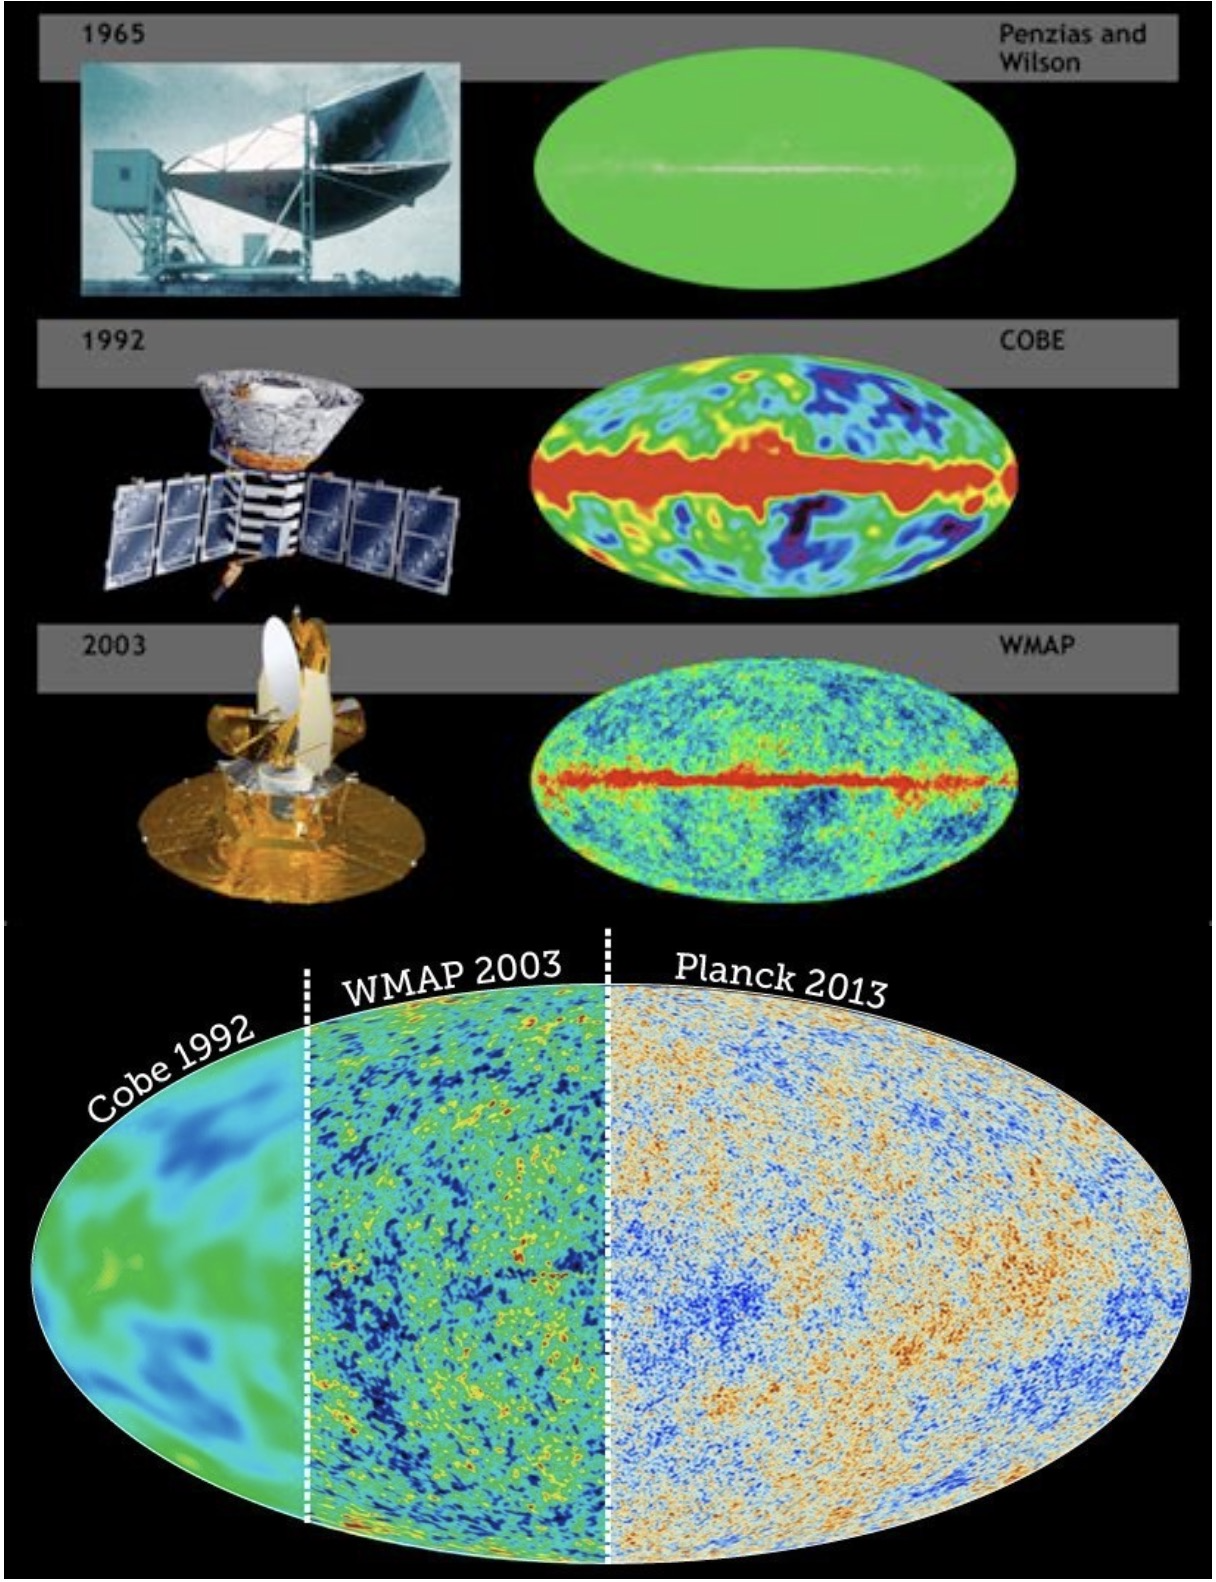
\includegraphics[width=0.5\columnwidth]{figures/cobe_wmap_planck.png}
\caption{The progression of CMB temperature anisotropy maps from COBE (1992) through WMAP (2003) to Planck (2013), illustrating the dramatic improvement in angular resolution and sensitivity over two decades of space-based observations.}
\label{fig:cmb_progression}
\end{figure}


% ===================================================================
\section{Mapping the Universe with Galaxy Surveys}
\label{sec:galaxy_surveys}
% ===================================================================

While the CMB provides a snapshot of the Universe at a redshift of $z\approx 1100$, galaxy redshift surveys map the three-dimensional distribution of matter in the more recent Universe. Constructing a redshift survey is a two-step process: first, a wide-field imaging survey identifies galaxies above a defined brightness limit; then, spectroscopic observations measure the redshifts of the selected galaxies.

\subsection*{Early Surveys and the Discovery of Cosmic Structure}

The first systematic redshift survey was the \textbf{CfA Redshift Survey}, begun in 1977 at the Center for Astrophysics. Its initial catalogue of approximately 2{,}200 galaxies, completed in 1982, was later extended to the CfA2 survey of 18{,}000 galaxies by John Huchra and Margaret Geller in the early 1990s. These pioneering surveys revealed that galaxies are not uniformly distributed, but instead trace a complex ``cosmic web'' of filaments, walls, and clusters surrounding large, nearly empty voids.

\begin{figure}[H]
\centering
% TODO: Add figure --- CfA redshift survey "stickman" map
%\fbox{\parbox{0.8\textwidth}{\centering\vspace{2cm}\textit{Figure placeholder: The CfA redshift survey slice showing the cosmic web}\vspace{2cm}}}
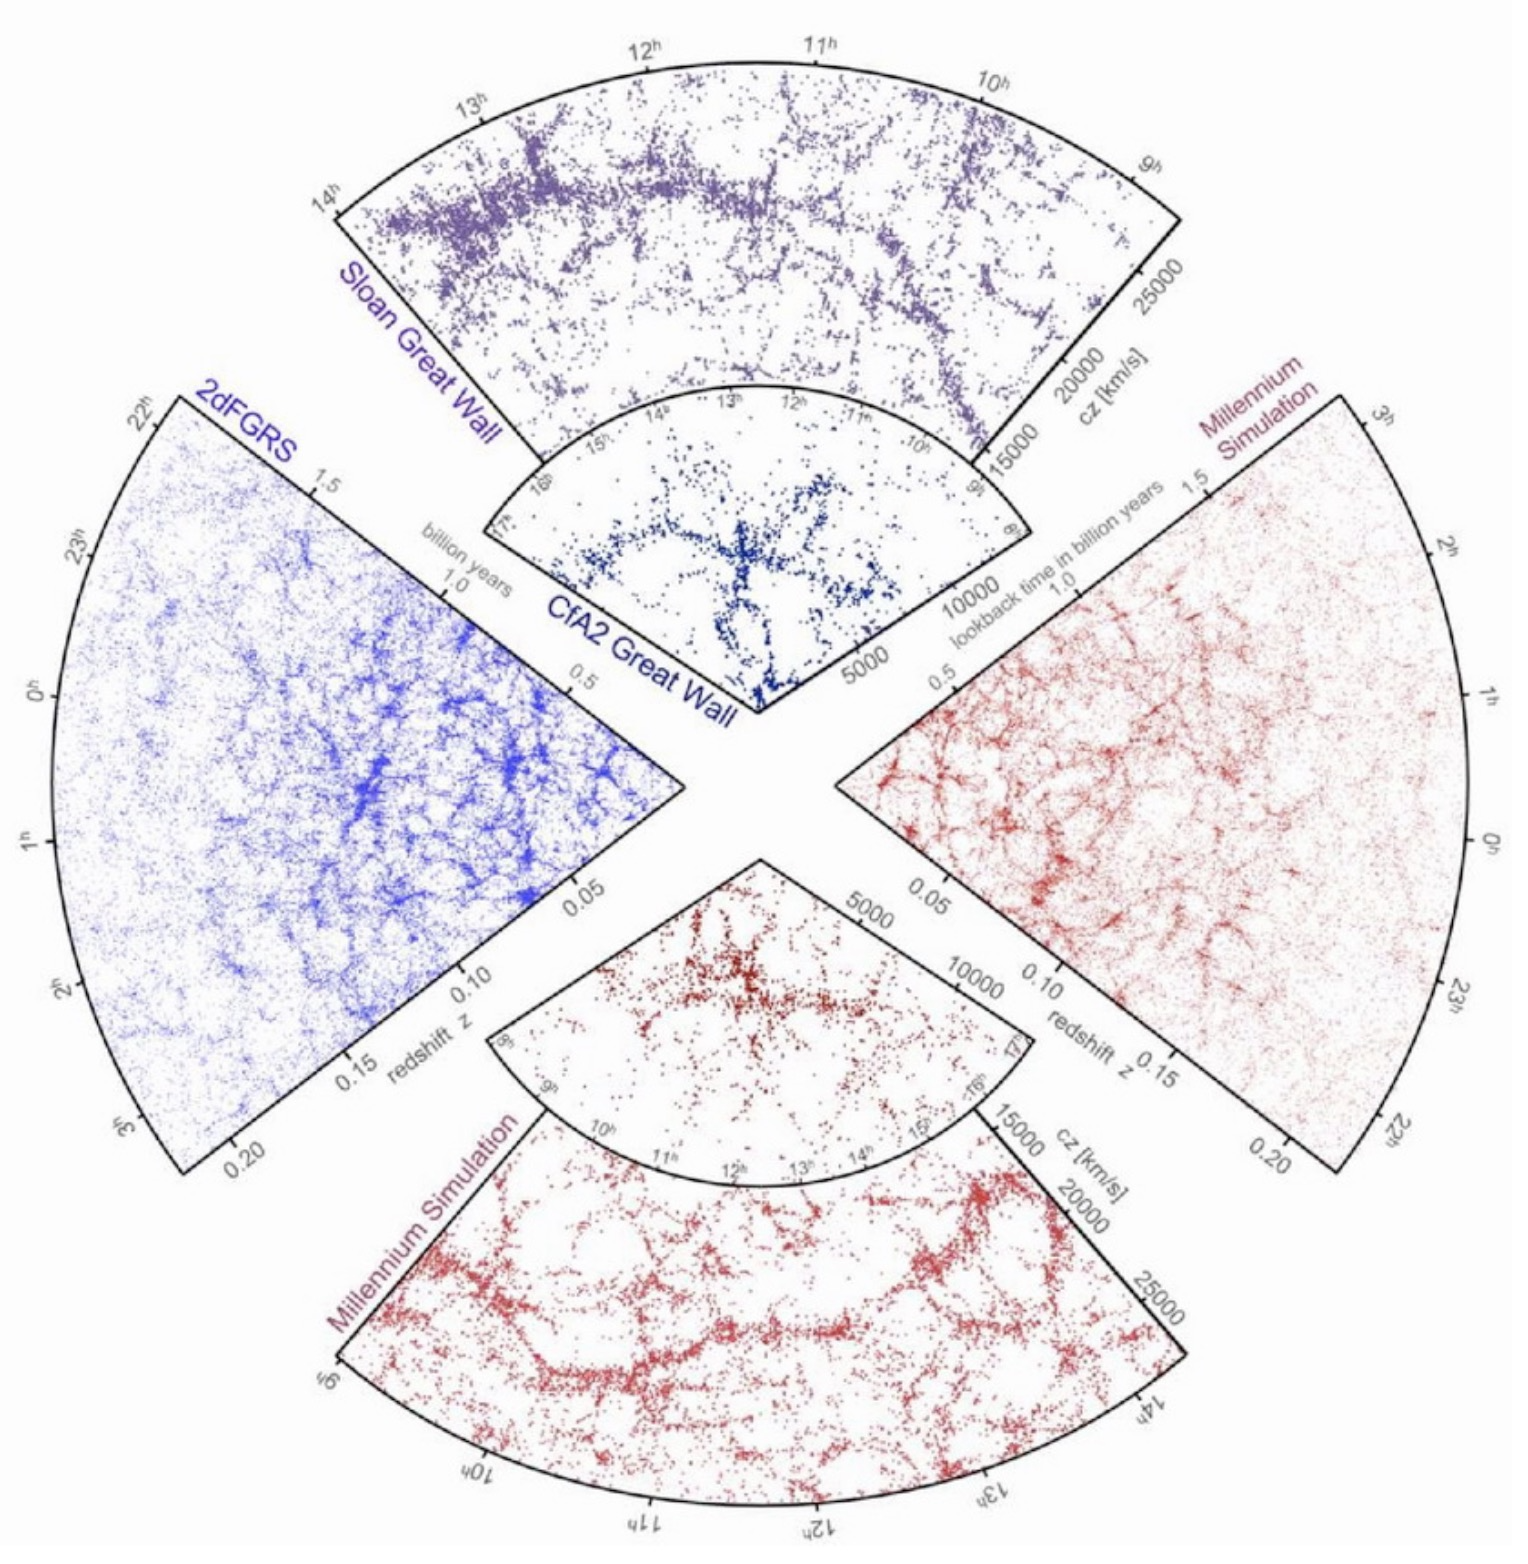
\includegraphics[width=0.6\columnwidth]{figures/2df_sdss.png}
\caption{A slice of the CfA2 redshift survey, revealing the filamentary large-scale structure of the Universe. Galaxies cluster on the surfaces of bubble-like voids.}
\label{fig:cfa_survey}
\end{figure}

\subsection*{The Multi-Fibre Revolution}

Early redshift surveys were limited by the need to observe one galaxy at a time. From the 1990s onwards, the development of fibre-optic multi-object spectrographs enabled the simultaneous measurement of hundreds of galaxy spectra, making much larger surveys feasible. Notable examples include:
\begin{itemize}
    \item \textbf{2dFGRS} (Two-degree-Field Galaxy Redshift Survey): 221{,}000 galaxy redshifts, completed in 2002.
    \item \textbf{SDSS} (Sloan Digital Sky Survey): The first large digital imaging and spectroscopic survey, which has mapped millions of galaxies and quasars since 2000.
\end{itemize}

In 2005, the 2dFGRS and SDSS collaborations independently reported the detection of the \textbf{baryon acoustic oscillation} (BAO) signal in the galaxy power spectrum---a characteristic scale imprinted by sound waves in the primordial plasma, providing a ``standard ruler'' for measuring cosmic distances. This opened a powerful new avenue for constraining the expansion history (see Chapter~\ref{ch:bao} for a detailed treatment).

\subsection*{BOSS, eBOSS, and DESI}

The SDSS programme continued with the \textbf{BOSS} (Baryon Oscillation Spectroscopic Survey, 2009--2014) and \textbf{eBOSS} (extended BOSS, 2014--2019) programmes, mapping the galaxy distribution across 11 billion years of cosmic history.

The current state of the art is the \textbf{Dark Energy Spectroscopic Instrument} (DESI), which began survey operations in 2021 and aims to measure approximately 35 million galaxy and quasar spectra---roughly ten times more than all previous surveys combined. DESI targets include luminous red galaxies (LRGs), emission line galaxies (ELGs), quasars (QSOs), and a bright galaxy survey (BGS), spanning a wide range of redshifts.

\begin{figure}[H]
\centering
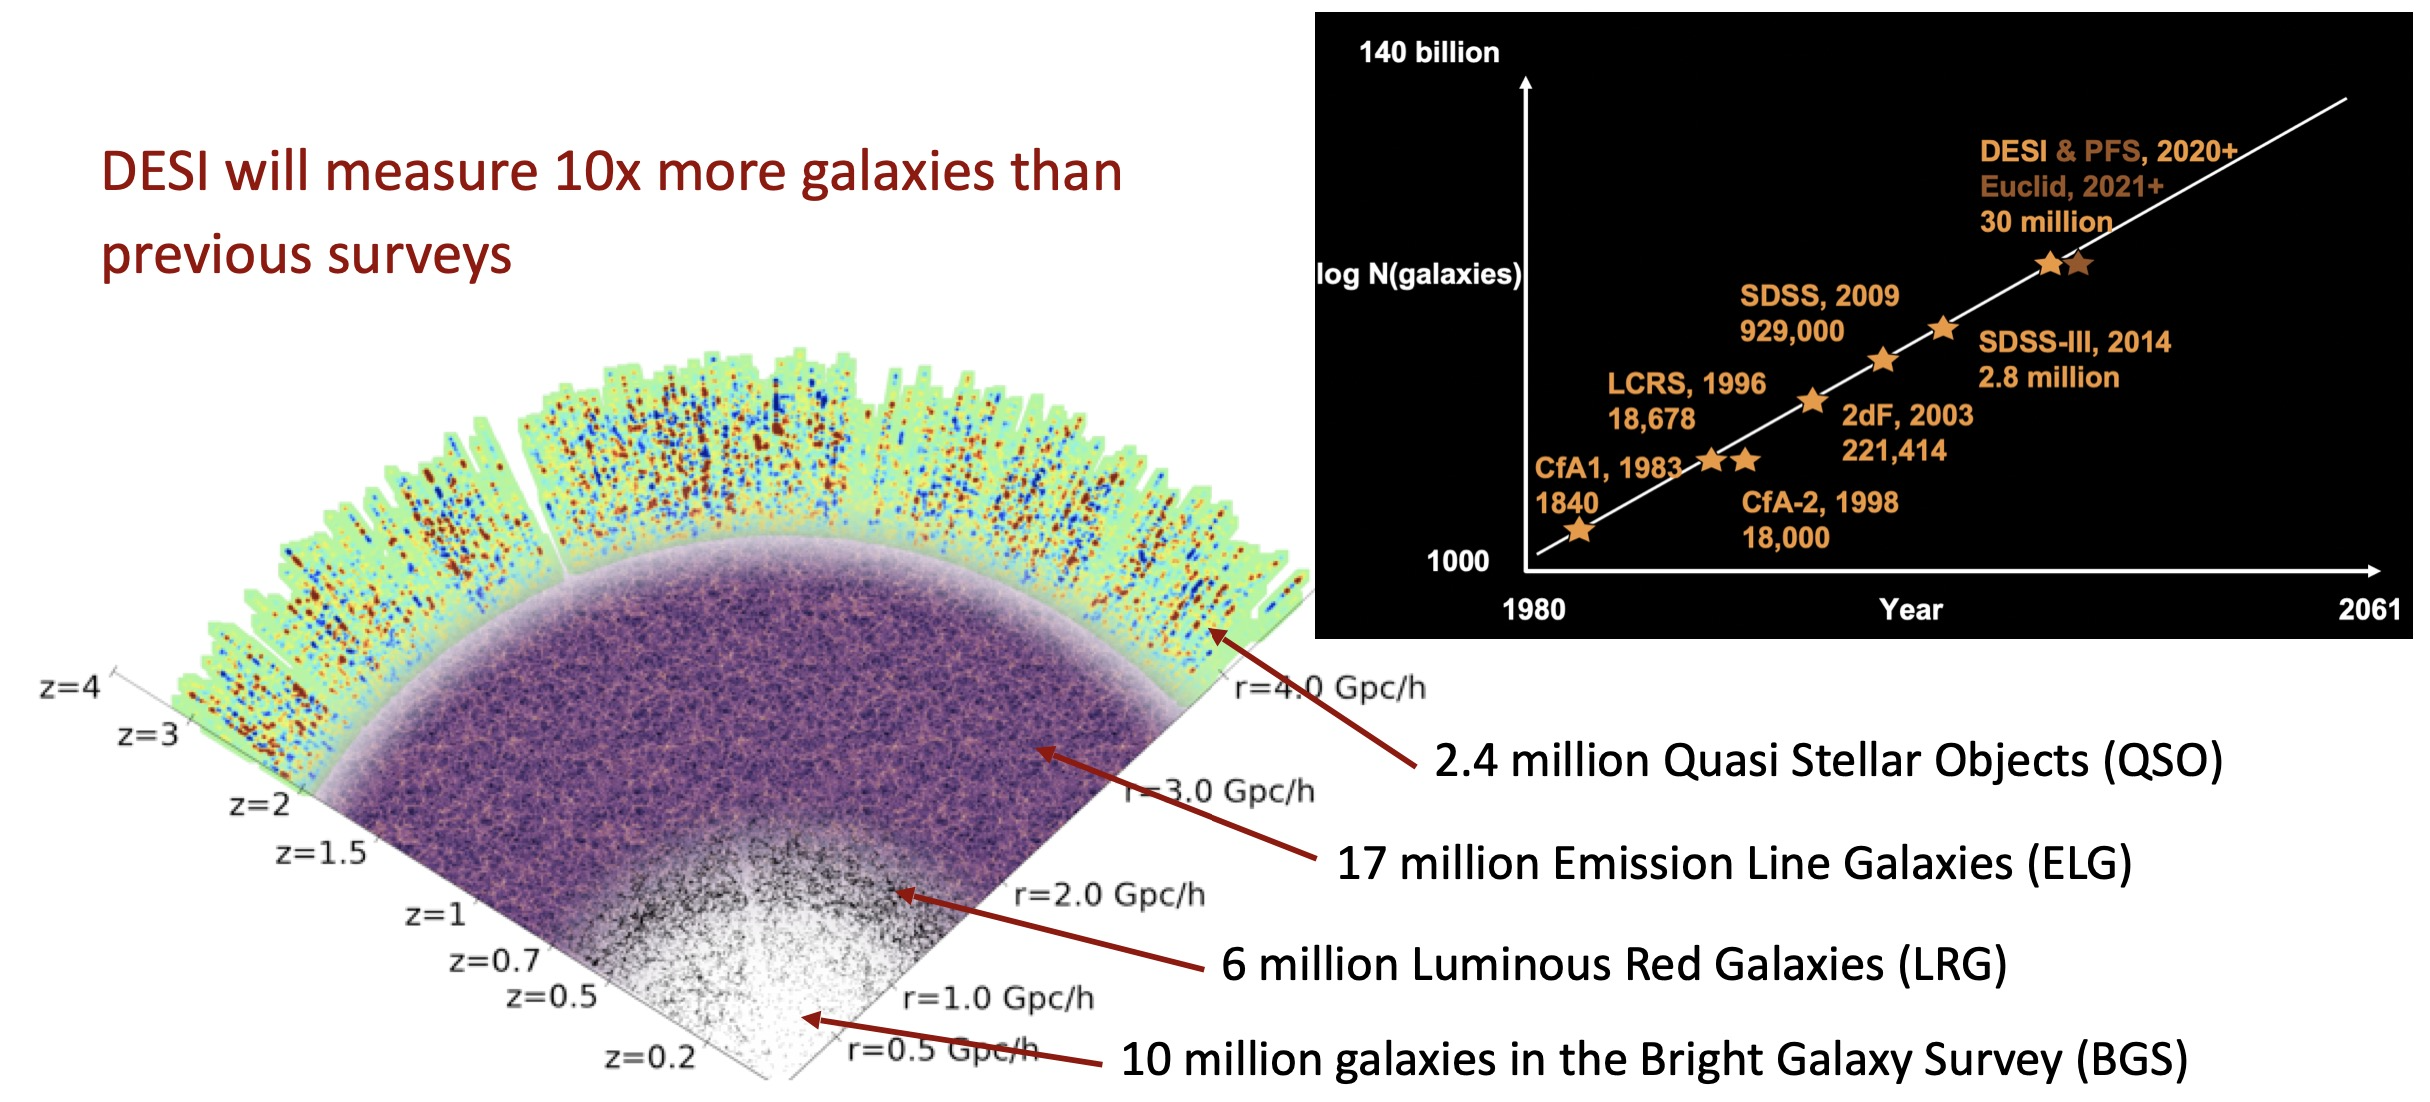
\includegraphics[width=0.8\columnwidth]{figures/desi.png}
\caption{A visualisation of the DESI survey volume, showing the distribution of different galaxy populations (LRGs, ELGs, QSOs) across redshift. DESI will measure approximately 35 million spectra, providing unprecedented precision on the expansion history and growth of structure.}
\label{fig:desi_survey}
\end{figure}


% ===================================================================
\section{Evidence for Dark Matter}
\label{sec:dark_matter_evidence}
% ===================================================================

The current cosmological picture requires two mysterious components that together account for roughly 95\% of the energy content of the Universe: dark matter and dark energy. We begin with the observational evidence for dark matter.

\subsection*{Galaxy Clusters and the Virial Theorem}

The first evidence for dark matter came from \textbf{Fritz Zwicky}'s study of the Coma Cluster (Abell~1656) in 1933. The Coma Cluster contains over 1{,}000 identified galaxies, and Zwicky measured their line-of-sight velocity dispersion. Applying the virial theorem, which relates the time-averaged kinetic and potential energies of a gravitationally bound system,
\begin{equation}
    \langle T \rangle = -\frac{1}{2}\langle U \rangle \quad\Longrightarrow\quad M \sim \frac{R\,\langle v^2\rangle}{G}\,,
\label{eq:virial}
\end{equation}
Zwicky estimated the total mass of the cluster and found it to be far larger than the luminous mass in its constituent galaxies. For the Coma Cluster, with a characteristic radius $R\approx 10^{23}\,\mathrm{m}$ and velocity dispersion $\langle v^2\rangle^{1/2}\approx 2\times 10^{6}\,\mathrm{m\,s^{-1}}$:
\begin{equation}
\boxed{M \approx \frac{R\,\langle v^2\rangle}{G} \sim \frac{2\times 10^{23}\times 4\times 10^{12}}{6.7\times 10^{-11}} \sim 10^{46}\,\mathrm{kg} \sim 5\times 10^{15}\,\Msun\,.}
\label{eq:coma_mass}
\end{equation}
This is far more mass than can be accounted for by the visible galaxies. Zwicky concluded that the cluster must be held together by some unseen ``dunkle Materie'' (dark matter). It would take approximately fifty years for the concept of dark matter to gain widespread acceptance.

\subsection*{Galaxy Rotation Curves}

In the late 1950s, observational hints emerged that stars in spiral galaxies were not moving as expected from Newtonian dynamics applied to the visible matter alone. In 1970, Vera Rubin, using a sensitive spectrograph developed by Kent Ford, measured the rotation velocities of stars at various distances from the centre of the Andromeda Galaxy (M31). For a galaxy whose mass is concentrated within radius $r$, Newtonian gravity predicts a Keplerian decline in the circular velocity:
\begin{equation}
    v_{\mathrm{circ}}(r) = \sqrt{\frac{GM(<r)}{r}} \;\propto\; r^{-1/2} \quad\text{(for $r$ beyond the luminous disc)}\,.
\end{equation}
Instead, Rubin found that rotation curves remain \textit{flat} ($v_{\mathrm{circ}}\approx\mathrm{const.}$) out to the largest measured radii, implying that $M(<r)\propto r$---the enclosed mass continues to grow linearly well beyond the visible disc. This is naturally explained by a massive, extended \textbf{dark matter halo} surrounding the galaxy.

\begin{figure}[H]
\centering
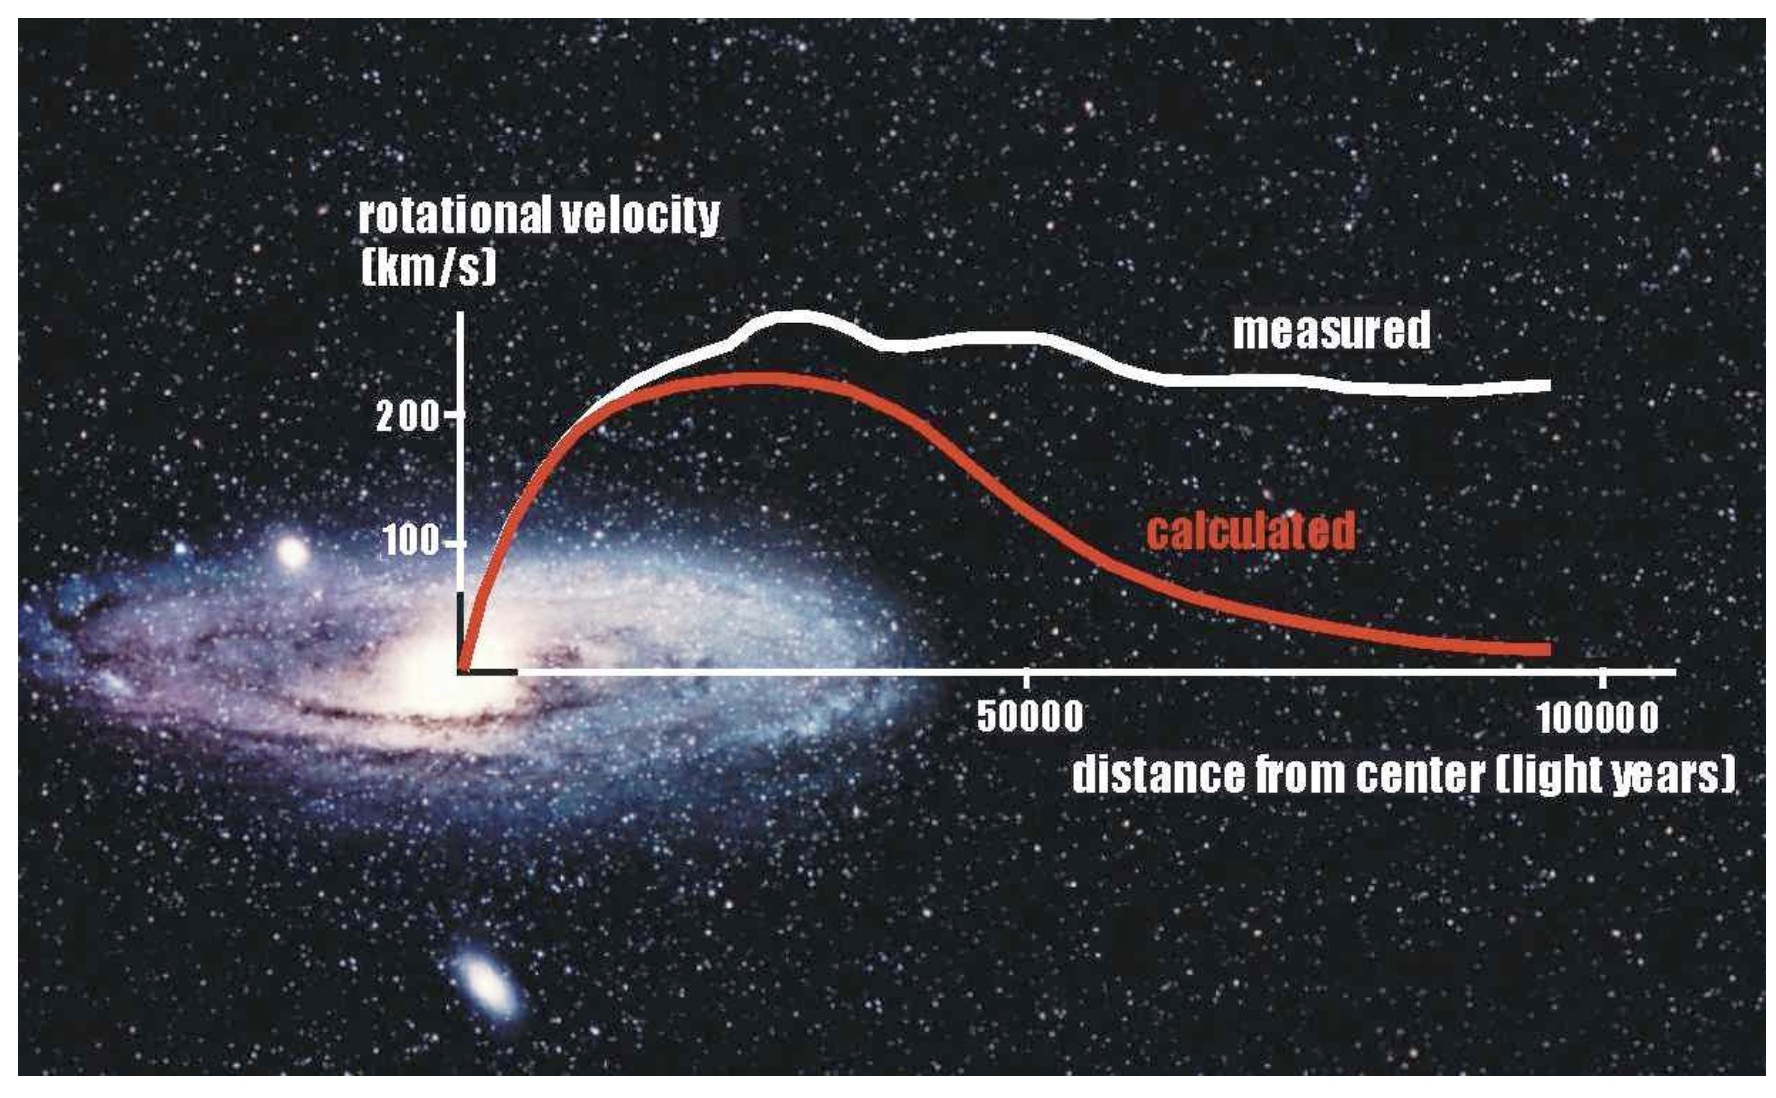
\includegraphics[width=0.6\columnwidth]{figures/rotation_curves.png}
\caption{Schematic galaxy rotation curve. The red line shows the expected Keplerian decline ($v\propto r^{-1/2}$) if only the visible disc mass were present. The white line shows the observed flat rotation curve, implying the existence of a dark matter halo whose enclosed mass grows linearly with radius.}
\label{fig:rotation_curve}
\end{figure}

\subsection*{Gravitational Lensing}

General relativity predicts that mass curves spacetime and deflects the paths of light rays. Massive objects such as galaxy clusters act as gravitational lenses, distorting the images of background galaxies. The strength of this lensing depends on the total projected mass along the line of sight, regardless of whether that mass is luminous or dark. Observations of both strong lensing (multiple images and arcs) around individual clusters and \textbf{weak lensing} (statistical distortions of the shapes of large samples of background galaxies) consistently require more mass than is observed in luminous matter, providing an independent confirmation of dark matter. We will study the physics of gravitational lensing in detail in Chapter~\ref{ch:gravitational_lensing}.

\begin{figure}[H]
\centering
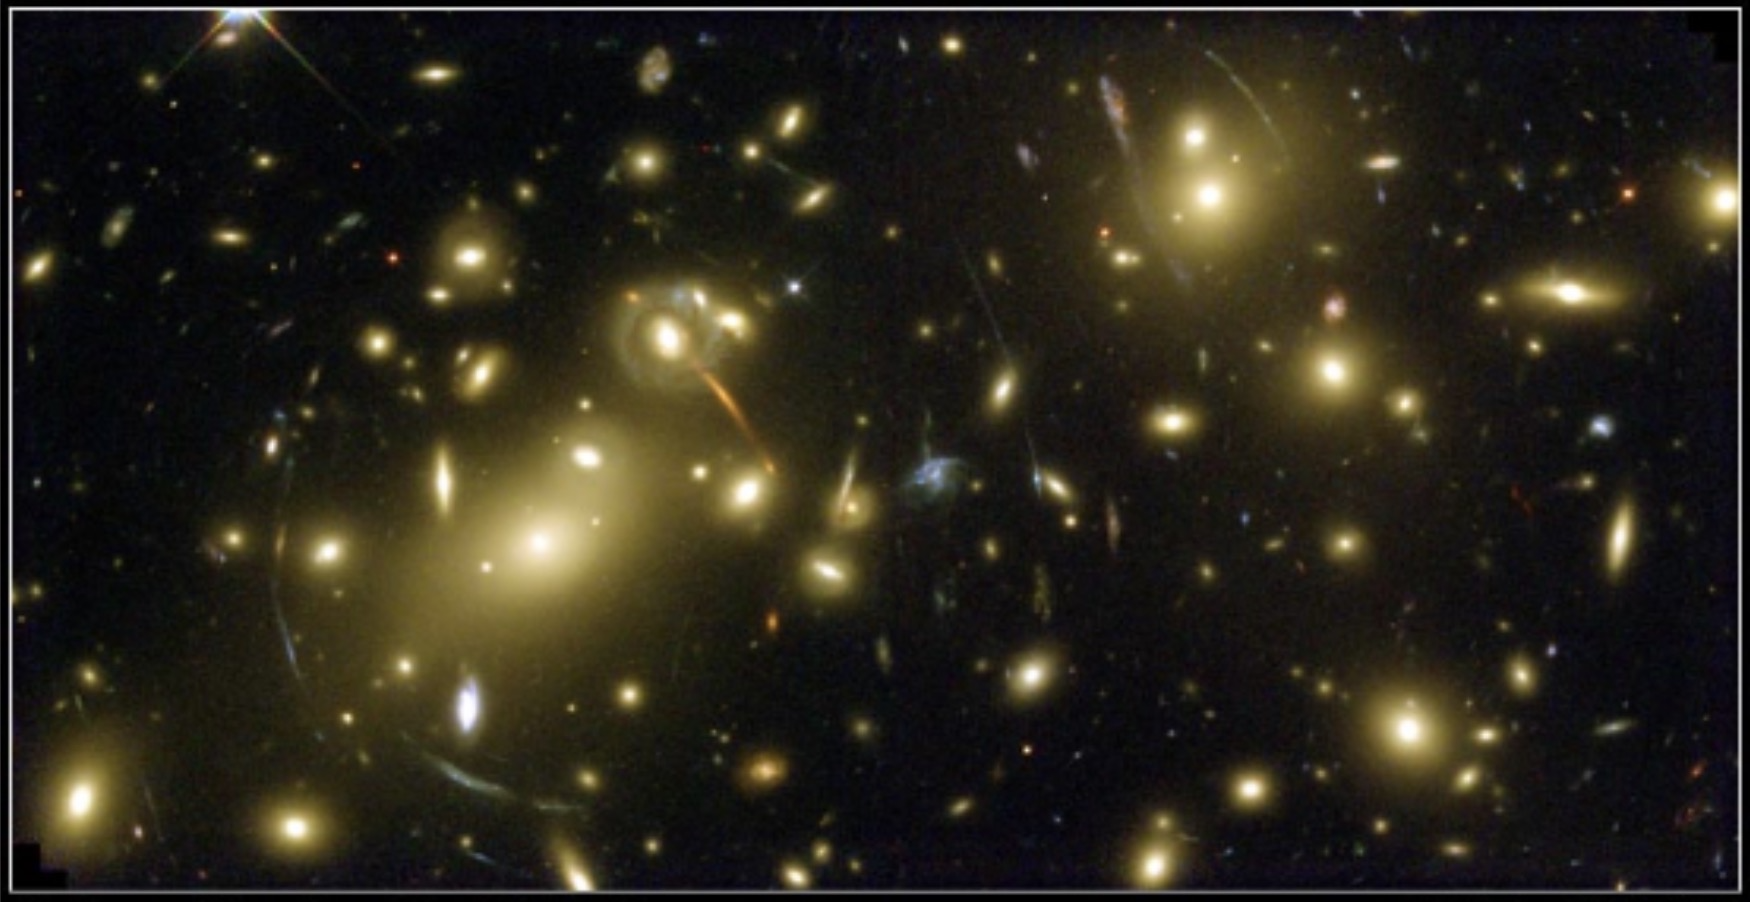
\includegraphics[width=0.7\columnwidth]{figures/abell_lensing.png}
\caption{Gravitational lensing by a massive galaxy cluster Abell 2218. The arcs visible around the cluster core are the distorted images of background galaxies, lensed by the cluster's gravitational field. The total lensing mass far exceeds the mass of the visible cluster galaxies and hot intracluster gas, providing strong evidence for dark matter.}
\label{fig:gravitational_lensing}
\end{figure}

\subsection*{The Cosmic Microwave Background}

The CMB provides yet another independent line of evidence for dark matter. In the early Universe, ordinary (baryonic) matter was ionised and interacted strongly with radiation through Thomson scattering, whereas dark matter interacts only gravitationally. These two components therefore evolve differently: baryons and photons form a tightly coupled fluid that supports acoustic oscillations, while dark matter perturbations grow freely under gravity, creating the gravitational potential wells into which the baryon--photon fluid falls.

This difference leaves a distinctive signature in the CMB power spectrum. Increasing the fraction of dark matter relative to baryonic matter changes the relative heights of the odd and even acoustic peaks. The Planck satellite's exquisite measurement of the CMB power spectrum constrains the dark matter density to $\Omc h^2 = 0.120 \pm 0.001$, roughly five times the baryon density $\Omb h^2 = 0.0224 \pm 0.0001$ (see Chapter~\ref{ch:cmb} for a full discussion).

%\begin{figure}[H]
%\centering
% TODO: Add figure --- CMB power spectrum with and without dark matter
%\fbox{\parbox{0.8\textwidth}{\centering\vspace{2cm}\textit{Figure placeholder: CMB temperature power spectrum with and without dark matter}\vspace{2cm}}}
%\caption{Comparison of the CMB temperature power spectrum in a universe with dark matter (left) and without dark matter (right). The presence of dark matter dramatically affects the relative heights and positions of the acoustic peaks.}
%\label{fig:cmb_dark_matter}
%\end{figure}


% ===================================================================
\section{Evidence for Dark Energy}
\label{sec:dark_energy_evidence}
% ===================================================================

\subsection*{Type Ia Supernovae}

Type Ia supernovae (SNe Ia) are thermonuclear explosions of white dwarf stars that reach a remarkably uniform peak luminosity, making them excellent ``standard candles'' for measuring cosmological distances. In 1998, two independent teams---the Supernova Cosmology Project and the High-$z$ Supernova Search Team---discovered that distant SNe Ia are systematically \emph{dimmer} than expected in a decelerating universe. The inescapable conclusion was that the expansion of the Universe is \emph{accelerating}, driven by an unknown component with negative pressure that has come to be called \textbf{dark energy}.

This discovery was awarded the Nobel Prize in Physics in 2011 (Saul Perlmutter, Brian Schmidt, and Adam Riess). It should be noted that there is ongoing investigation into potential systematic effects, in particular whether the peak brightness of SNe Ia correlates with the age of the host stellar population, which could affect cosmological inferences.

\begin{figure}[H]
\centering
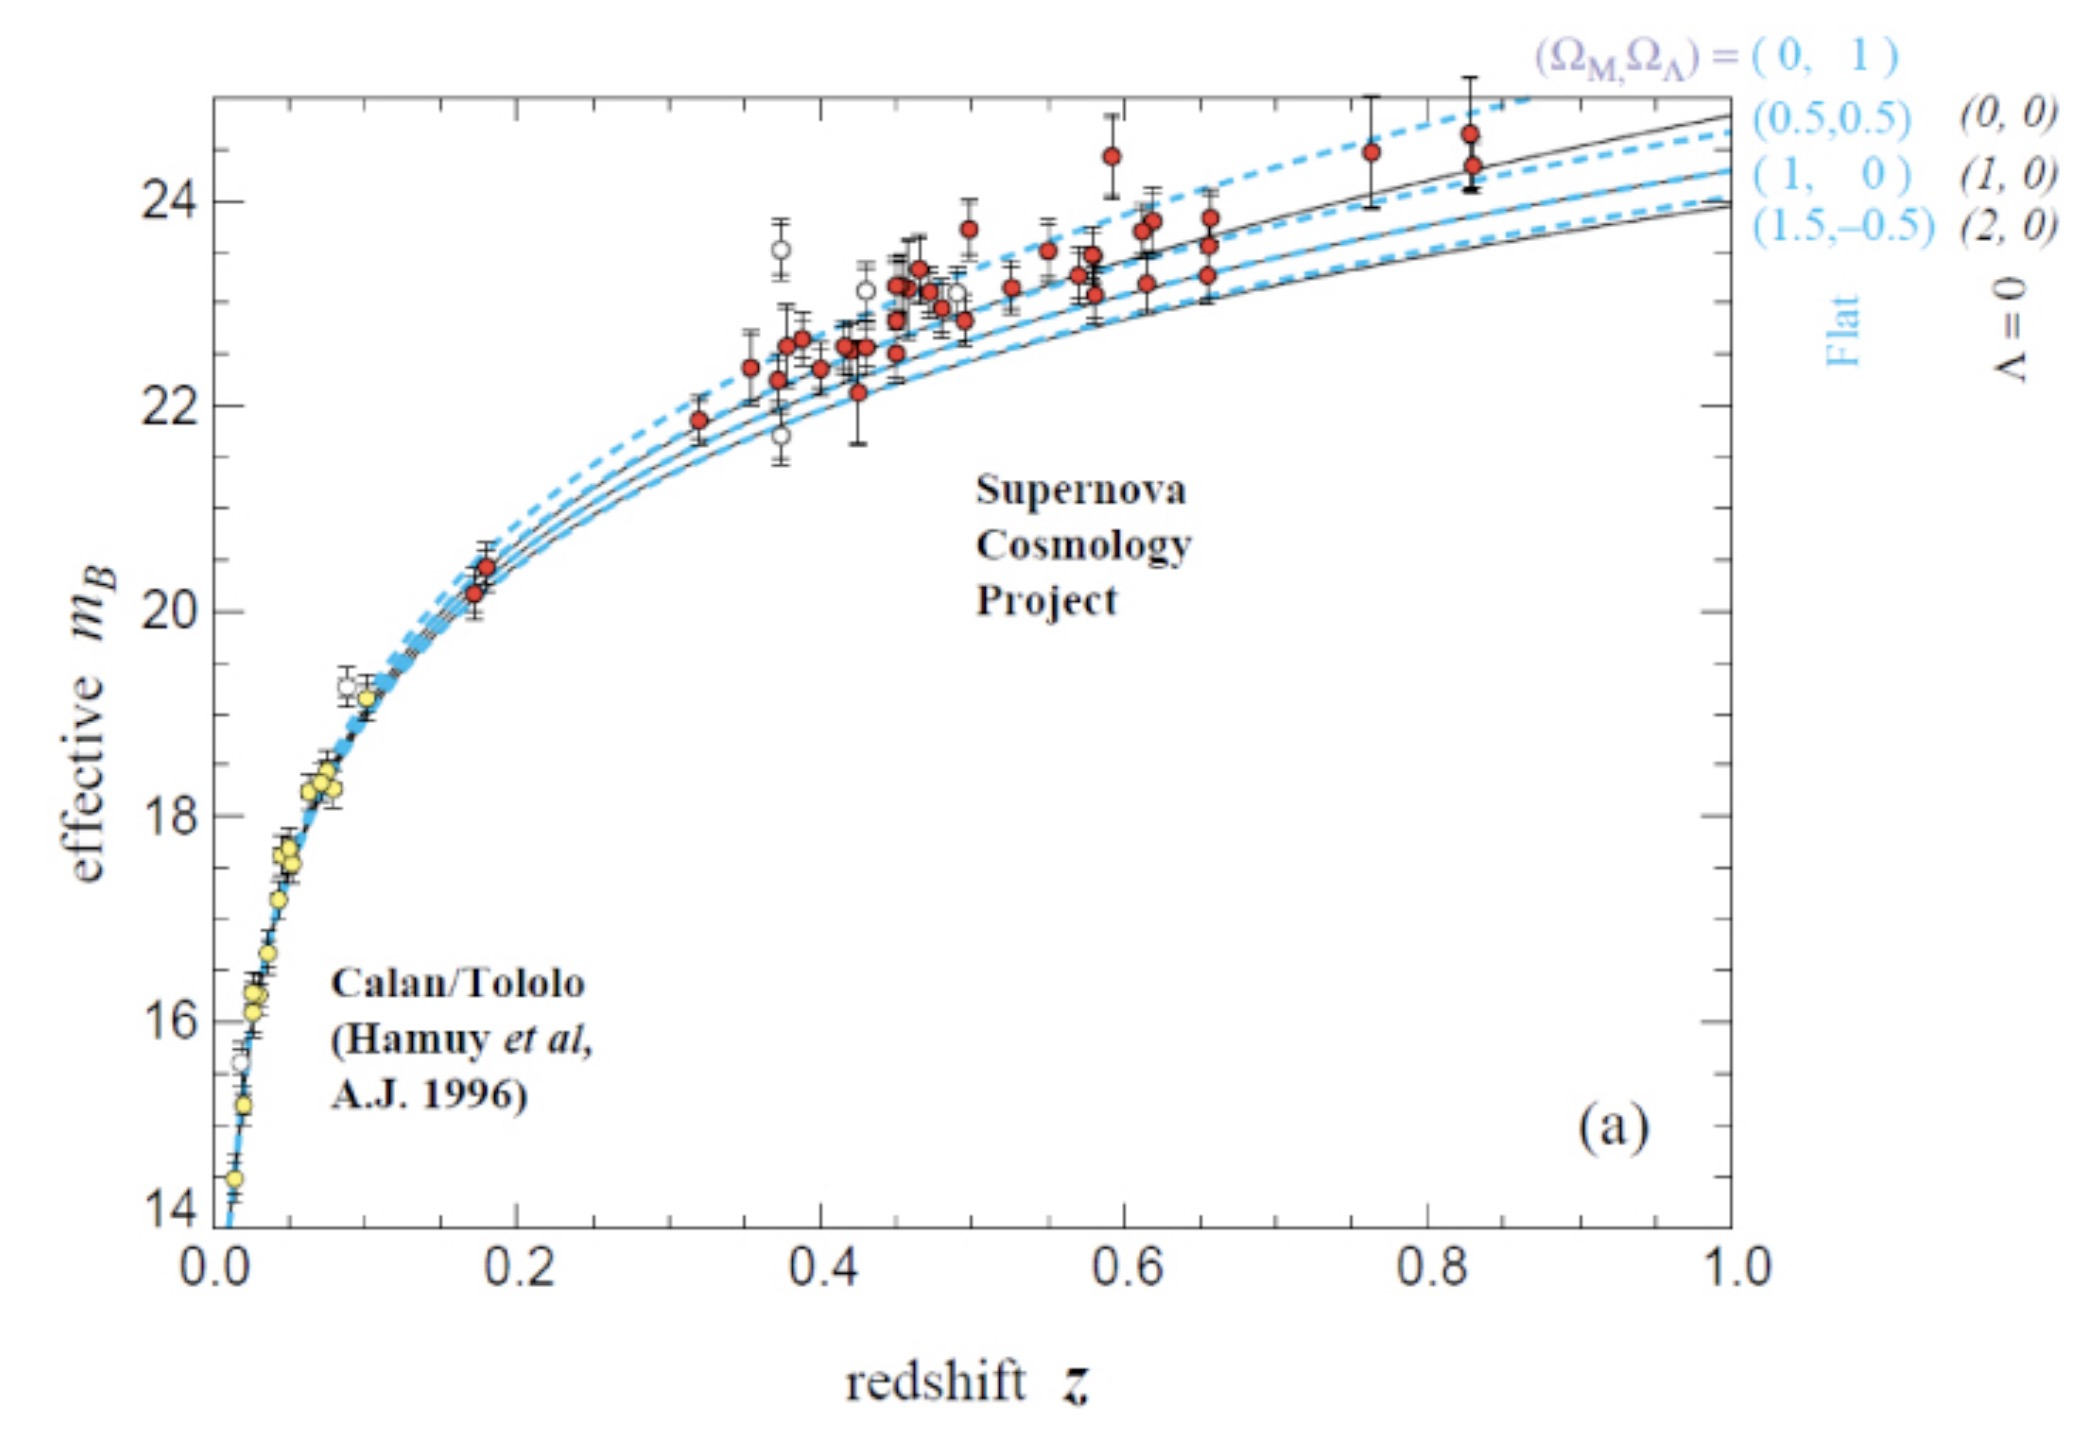
\includegraphics[width=0.6\columnwidth]{figures/supernovae_evidence.png}
\caption{The Hubble diagram for Type~Ia supernovae. Distant SNe~Ia are systematically fainter than expected in a matter-dominated, decelerating universe, providing direct evidence for the accelerating expansion.}
\label{fig:sn_hubble}
\end{figure}

\subsection*{CMB and the Geometry of Space}

Measurements of CMB anisotropies indicate that the Universe is spatially flat to high precision, meaning $\Omtot \approx 1$. However, the total amount of matter in the Universe (baryonic plus dark matter), as measured independently from the CMB power spectrum, accounts for only about 30\% of the critical density: $\Omm\approx 0.3$. For the Universe to be flat, the remaining $\sim 70\%$ must be supplied by an additional component: dark energy, with $\OmDE\approx 0.7$.

\begin{figure}[H]
\centering
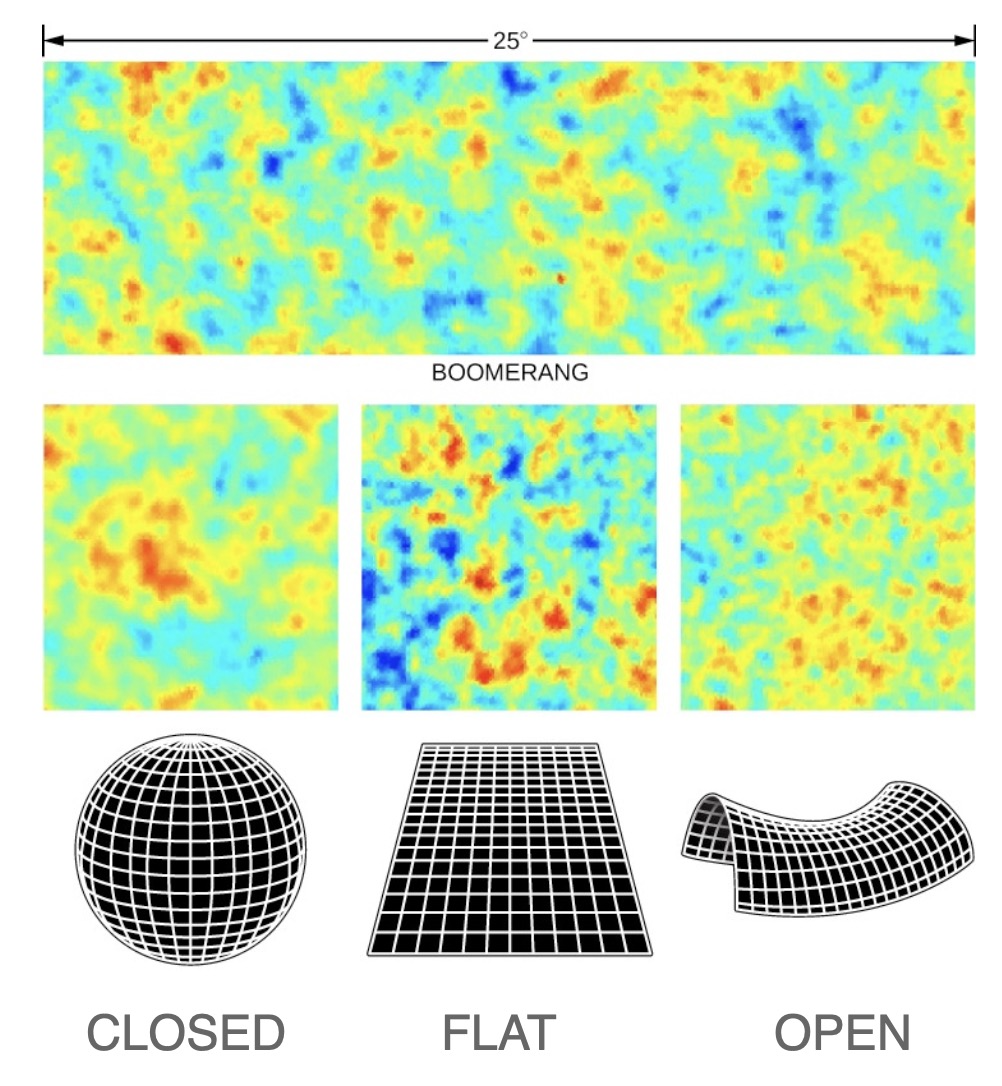
\includegraphics[width=0.6\columnwidth]{figures/cmb_curvature.png}
\caption{The effect of spatial curvature on the apparent angular size of features in the CMB. In a closed universe, features appear larger; in an open universe, smaller. CMB observations strongly favour a flat geometry ($\Omtot \approx 1$).}
\label{fig:cmb_geometry}
\end{figure}

\subsection*{The Integrated Sachs--Wolfe Effect}

The \textbf{integrated Sachs--Wolfe (ISW) effect} provides a direct probe of dark energy through the CMB. The physical mechanism is as follows. As a CMB photon falls into a gravitational potential well (such as that associated with a supercluster), it gains energy (is blueshifted). While the photon traverses the structure, the Universe continues to expand, and if dark energy is present and causing the expansion to accelerate, the potential well decays during the photon's passage. When the photon climbs back out, the potential is shallower than when it fell in, so the photon loses less energy climbing out than it gained falling in. The result is a net energy gain---a small temperature increase on the CMB in the direction of the supercluster. The reverse occurs for voids: photons crossing an underdensity experience a net energy loss.

Observationally, this is detected by cross-correlating the positions of large-scale structures (superclusters and voids) identified in galaxy surveys with the CMB temperature map. The detection of a positive correlation---hotter CMB in the direction of overdensities and cooler CMB toward voids---provides evidence for the decay of gravitational potentials, which in a matter-dominated universe would not occur. The ISW effect is therefore a signature of dark energy or, more generally, of any departure from matter domination at late times.

\begin{figure}[H]
\centering
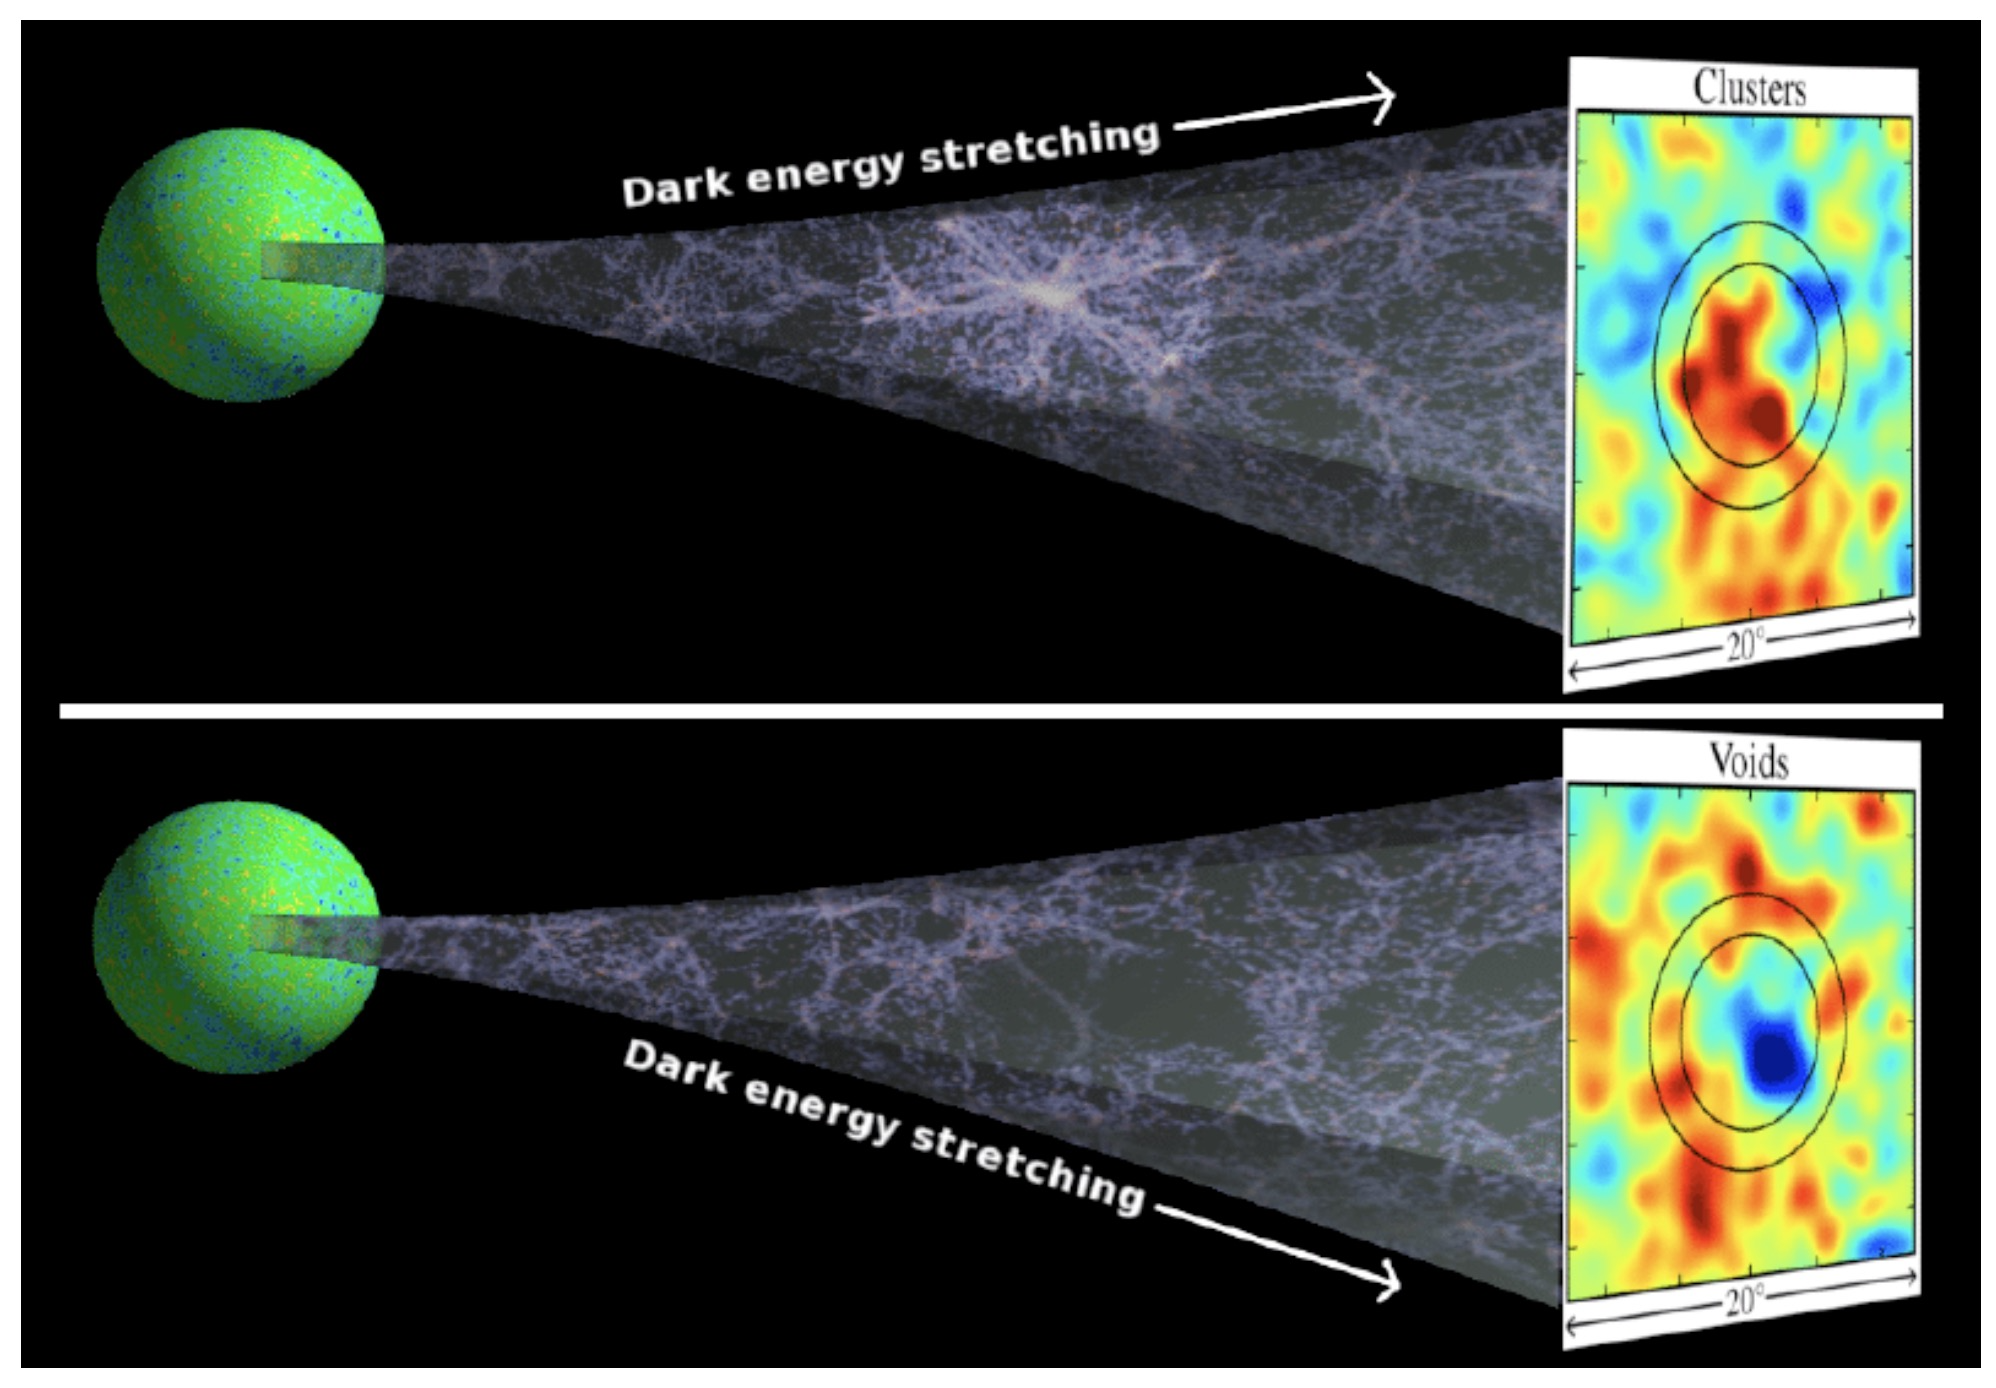
\includegraphics[width=0.7\columnwidth]{figures/sachs_wolfe.png}
\caption{Schematic illustration of the integrated Sachs--Wolfe (ISW) effect. A photon falling into a gravitational potential well gains energy. During transit, the accelerating expansion stretches the potential, so the photon loses less energy climbing out than it gained falling in. The net effect is a slight temperature increase toward superclusters and a decrease toward voids.}
\label{fig:isw_effect}
\end{figure}

\subsection*{Baryon Acoustic Oscillations}

Baryon acoustic oscillations (BAO) provide a powerful geometric probe of the expansion history. The BAO signal---a characteristic excess of galaxy pairs separated by approximately $150\,\mathrm{Mpc}$---acts as a standard ruler that can be measured at different redshifts to constrain both the angular diameter distance $D_A(z)$ and the Hubble parameter $H(z)$.

Combined BAO measurements from SDSS, BOSS, and eBOSS yield a detection of dark energy at greater than $8\sigma$ significance from BAO data alone, independent of any supernova or CMB data. When combined with CMB constraints and the supernova Hubble diagram, the BAO measurements provide some of the tightest constraints on the dark energy equation of state (see Chapter~\ref{ch:bao}).

\begin{figure}[H]
\centering
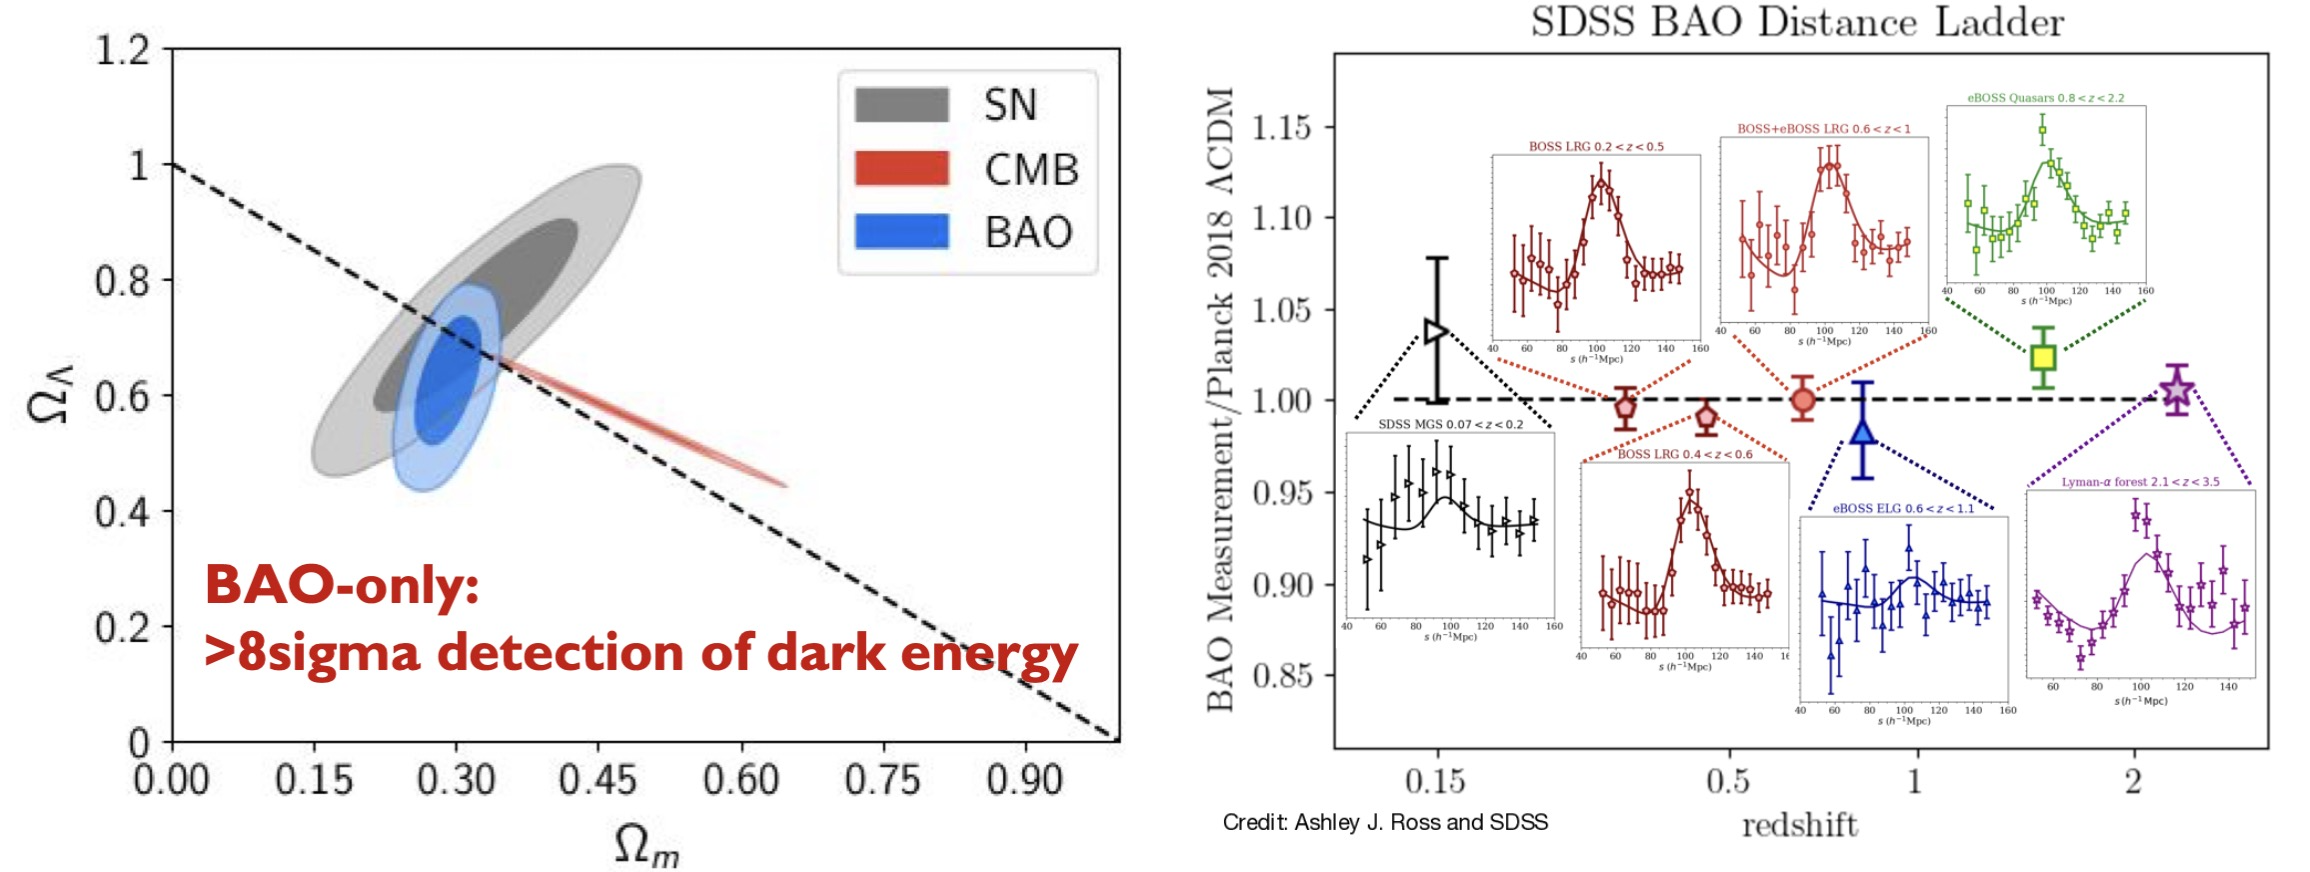
\includegraphics[width=0.7\columnwidth]{figures/bao_DE.png}
\caption{Constraints on the dark energy density from BAO measurements alone (SDSS/BOSS/eBOSS), demonstrating a detection of dark energy at greater than $8\sigma$ significance, independent of supernova or CMB data.}
\label{fig:bao_constraints}
\end{figure}


% ===================================================================
\section{The Cosmic Energy Budget}
\label{sec:energy_budget}
% ===================================================================

Combining all the observational probes described above---CMB, galaxy clustering, supernovae, gravitational lensing---gives us a remarkably consistent picture of the composition of the Universe:
\begin{itemize}
    \item \textbf{Ordinary (baryonic) matter}: approximately 5\% of the total energy density. This includes all atoms, stars, planets, gas, and dust.
    \item \textbf{Dark matter}: approximately 25\%. A non-luminous, non-baryonic component that interacts gravitationally but not electromagnetically.
    \item \textbf{Dark energy}: approximately 70\%. A component with negative pressure driving the accelerated expansion of the Universe.
\end{itemize}
Taken together, approximately 95\% of the energy content of the Universe is in forms that are not described by the Standard Model of particle physics. This is both humbling and exciting: the Universe is largely composed of substances whose fundamental nature remains unknown.

\begin{figure}[H]
\centering
% TODO: Add figure --- Cosmic energy budget pie chart
%\fbox{\parbox{0.8\textwidth}{\centering\vspace{2cm}\textit{Figure placeholder: Pie chart of the cosmic energy budget (5\% baryons, 25\% dark matter, 70\% dark energy)}\vspace{2cm}}}
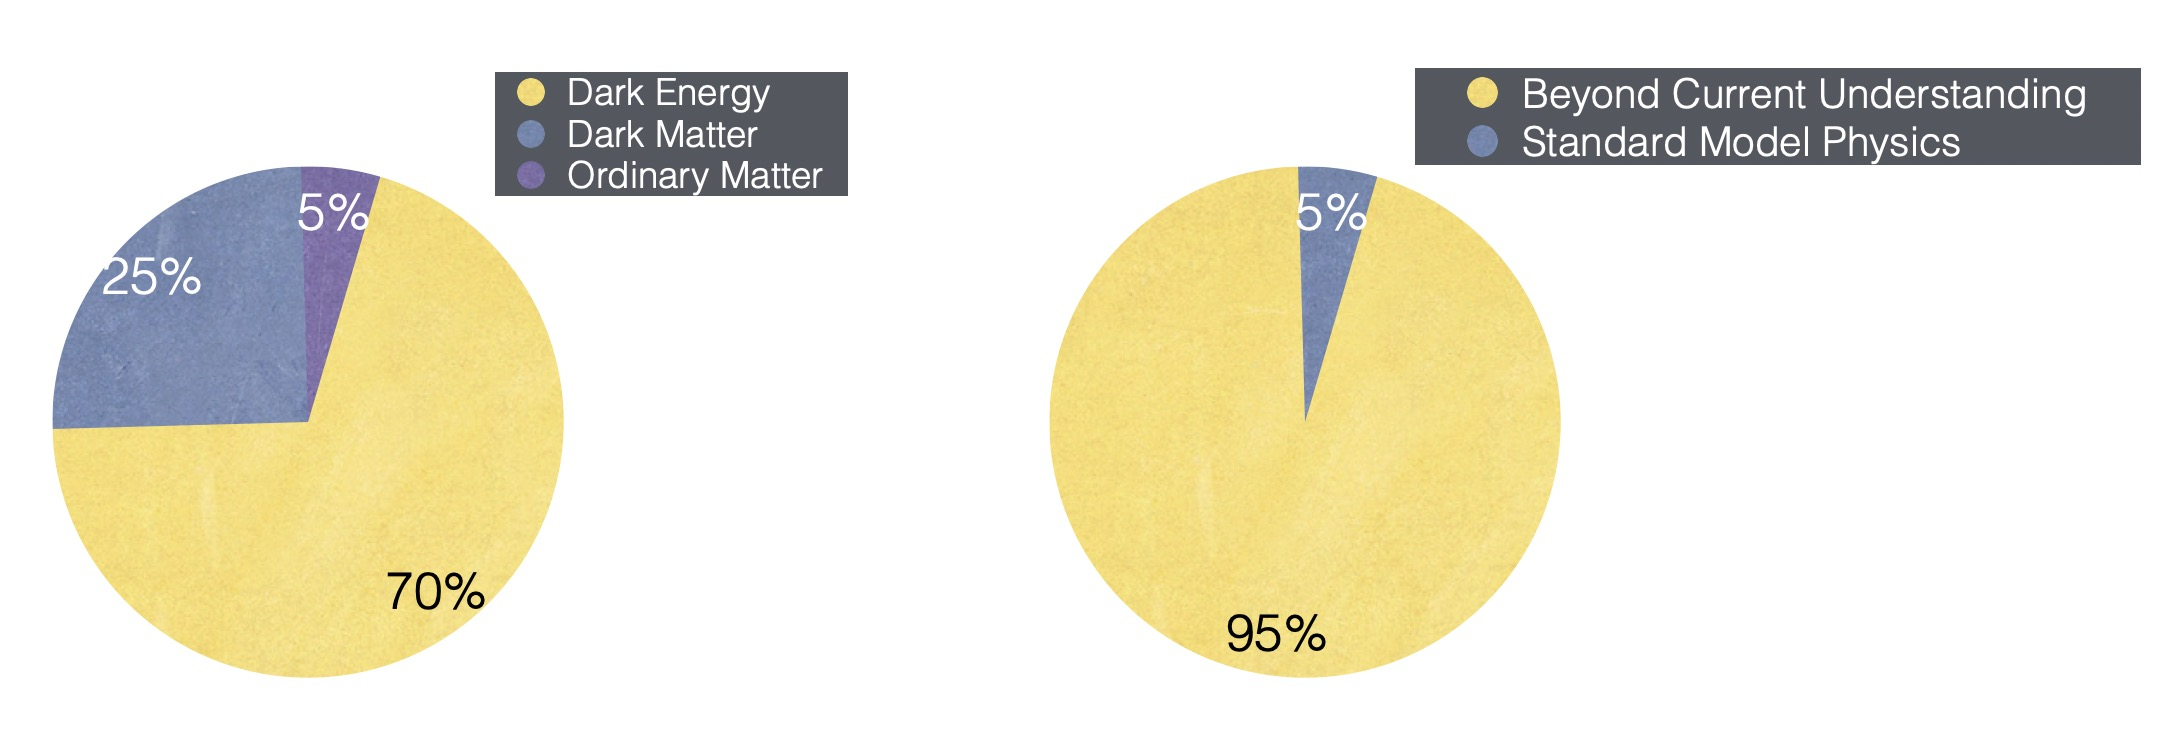
\includegraphics[width=\columnwidth]{figures/cosmic_pie.png}
\caption{The cosmic energy budget. Ordinary baryonic matter accounts for only about 5\% of the total energy density. Dark matter contributes roughly 25\%, and dark energy roughly 70\%. Approximately 95\% of the Universe is in forms not described by the Standard Model of particle physics.}
\label{fig:energy_budget}
\end{figure}


% ===================================================================
\section{Open Questions and Current Controversies}
\label{sec:open_questions}
% ===================================================================

The $\Lcdm$ model---a spatially flat universe with a cosmological constant ($\Lambda$) plus cold dark matter (CDM), described by just six free parameters---fits an impressive range of cosmological data: the CMB power spectrum, BAO, SNe Ia, gravitational lensing, and galaxy cluster counts. With only six numbers, plus some well-motivated assumptions, we can account for observations spanning 13.8 billion years of cosmic history. This is a remarkable achievement. However, several open questions and emerging tensions suggest that our understanding may be incomplete.

\subsection*{What is Dark Matter?}

The nature of dark matter remains one of the greatest unsolved problems in physics. A wide range of candidates have been proposed:
\begin{itemize}
    \item \textbf{Weakly Interacting Massive Particles (WIMPs)}: Motivated by supersymmetry and other beyond-Standard-Model theories. Extensive direct detection experiments have so far yielded null results, placing increasingly stringent limits on the WIMP--nucleon cross section.
    \item \textbf{Axions and axion-like particles}: Light bosonic particles originally proposed to solve the strong CP problem in quantum chromodynamics. Dedicated experiments such as ADMX are searching for axion signals.
    \item \textbf{Sterile neutrinos}: Hypothetical right-handed neutrinos that could serve as warm dark matter candidates.
    \item \textbf{Primordial black holes (PBHs)}: Black holes formed in the early Universe, potentially in a mass range not yet excluded by observations.
    \item \textbf{MACHOs} (Massive Compact Halo Objects): Baryonic objects such as brown dwarfs or black holes. Microlensing surveys have largely ruled out MACHOs as the dominant component of dark matter.
    \item \textbf{Modified gravity}: Alternatives such as Modified Newtonian Dynamics (MOND), Tensor--Vector--Scalar gravity (TeVeS), and entropic gravity attempt to explain dark matter phenomenology by modifying the law of gravity rather than introducing new particles. These models face significant challenges in explaining the full range of cosmological observations.
\end{itemize}

%\begin{figure}[H]
%\centering
% TODO: Add figure --- Dark matter candidates taxonomy
%\fbox{\parbox{0.8\textwidth}{\centering\vspace{2cm}\textit{Figure placeholder: Taxonomy of dark matter candidates}\vspace{2cm}}}
%\caption{A taxonomy of dark matter candidates, ranging from ultralight axions to primordial black holes, alongside modified gravity alternatives. The viable parameter space is being progressively constrained by direct detection, indirect detection, and collider experiments.}
%\label{fig:dm_candidates}
%\end{figure}

\subsection*{Reionisation and the Cosmic Dawn}

After recombination at $z\approx 1100$, the Universe entered the ``dark ages''---a period during which neutral hydrogen filled intergalactic space and no luminous sources existed. The formation of the first stars and galaxies at $z\sim 20$--$30$ began the process of \textbf{reionisation}, in which ultraviolet radiation from these first objects gradually ionised the intergalactic medium. The timing and topology of reionisation remain poorly constrained and are the subject of intensive observational efforts.

A particularly intriguing result came from the EDGES experiment, which in 2018 reported a detection of the global 21\,cm absorption signal from neutral hydrogen at $z\approx 17$, corresponding to the epoch when the first stars began illuminating the Universe. The absorption trough was deeper than expected, which, if confirmed, could point to exotic physics such as interactions between baryons and dark matter that cool the gas below the standard prediction.

\subsection*{The Hubble Tension}

Perhaps the most discussed discrepancy in modern cosmology is the \textbf{Hubble tension}: a persistent disagreement between two routes to measuring the present-day expansion rate~$\Hnot$.
\begin{itemize}
    \item \textbf{Early-universe route}: The Planck satellite's measurement of the CMB power spectrum, interpreted within the $\Lcdm$ model, yields $\Hnot = 67.4 \pm 0.5\kmsMpc$.
    \item \textbf{Late-universe route}: The SH0ES collaboration's calibration of the distance ladder using Cepheid variables and Type~Ia supernovae gives $\Hnot = 73.0 \pm 1.0\kmsMpc$.
\end{itemize}
The discrepancy is approximately $5\sigma$---far too large to be a statistical fluke. These two methods are measuring the same physical quantity; either one (or both) harbours an unidentified systematic error, or the $\Lcdm$ model is incomplete and new physics is required to reconcile them.

\begin{figure}[H]
\centering
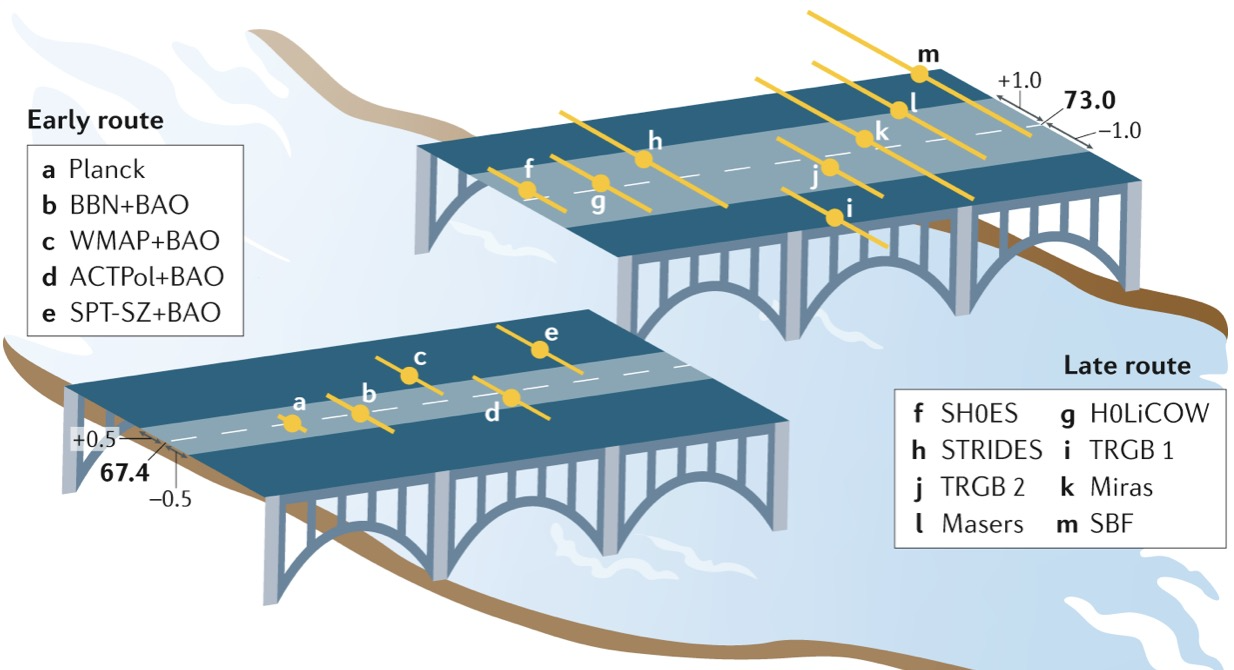
\includegraphics[width=0.8\columnwidth]{figures/H0_early_late.png}
\caption{Summary of $\Hnot$ measurements. Early-universe determinations (CMB, BAO) cluster around $67$--$68\kmsMpc$, while late-universe determinations (Cepheids, SNe~Ia, strong lensing time delays) cluster around $72$--$74\kmsMpc$. The $\sim 5\sigma$ discrepancy is the Hubble tension.}
\label{fig:hubble_tension}
\end{figure}

\subsection*{Evolving Dark Energy?}

The simplest model for dark energy is a cosmological constant~$\Lambda$ with a constant equation of state $w = -1$. However, recent results from the DESI collaboration, combining BAO measurements with various supernova samples, show hints of tension with this simple picture. When the dark energy equation of state is allowed to vary with time using the CPL parametrisation $w(a) = w_0 + w_a(1-a)$, the data show a preference for $w_0 > -1$ and $w_a < 0$---that is, dark energy that was less negative in the past and has become more negative over time. When CMB constraints from Planck are added, the preference for time-varying dark energy strengthens.

These results are tantalising but not yet conclusive. Systematic effects in the supernova samples---including a potential correlation between supernova peak brightness and the age of the host galaxy's stellar population---are being actively investigated. Future DESI data releases, combined with next-generation supernova surveys, will clarify whether dark energy truly evolves.

\begin{figure}[H]
\centering
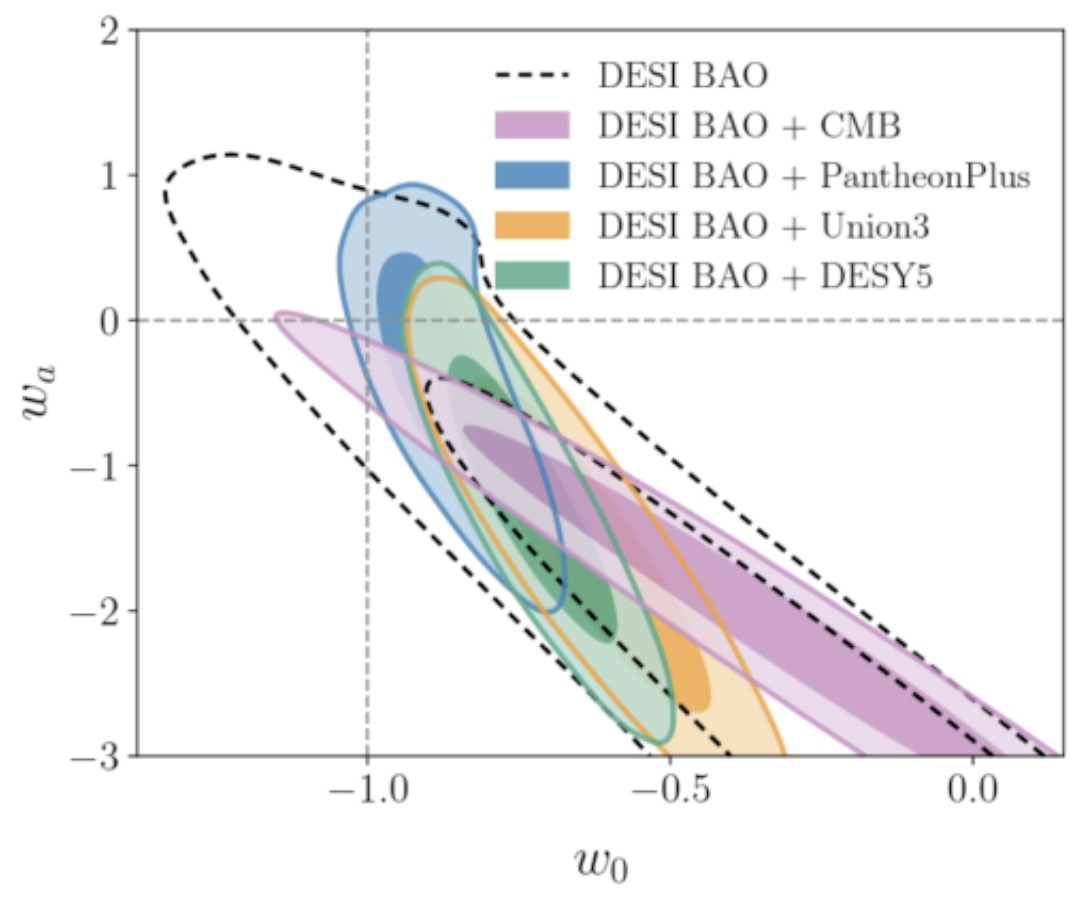
\includegraphics[width=0.7\columnwidth]{figures/w0_bao_sne.png}
\caption{Constraints on the dark energy equation of state parameters $w_0$ and $w_a$ from DESI BAO data combined with various supernova samples and Planck CMB data. The cosmological constant ($w_0=-1$, $w_a=0$) lies at the edge of the allowed region, suggesting possible time evolution of dark energy.}
\label{fig:desi_de}
\end{figure}

\subsection*{The $\sigmaEight$ Tension}

A second, less dramatic but persistent, discrepancy has emerged in the amplitude of matter density fluctuations, characterised by the parameter $\sigmaEight$ (the root-mean-square fluctuation in spheres of radius $8\,h^{-1}\,\mathrm{Mpc}$). The value inferred from the CMB (assuming $\Lcdm$) is somewhat higher than that measured directly from weak gravitational lensing surveys at lower redshift. Although the significance is currently $2$--$3\sigma$---less alarming than the Hubble tension---it may point to the same underlying issue: either unaccounted-for systematics or a departure from $\Lcdm$.

%\begin{figure}[H]
%\centering
% TODO: Add figure --- sigma_8 tension plot
%\fbox{\parbox{0.8\textwidth}{\centering\vspace{2cm}\textit{Figure placeholder: $\sigmaEight$ measurements from CMB vs.\ weak lensing surveys}\vspace{2cm}}}
%\caption{Comparison of $\sigmaEight$ (or the related quantity $S_8 = \sigmaEight\sqrt{\Omm/0.3}$) as measured from the CMB (Planck) and from weak lensing surveys (KiDS, DES, HSC). The CMB-inferred value is consistently higher than the direct low-redshift measurements.}
%\label{fig:sigma8_tension}
%\end{figure}

\subsection{Paradigm Shifts in Cosmology}

The philosopher of science Thomas Kuhn, in \textit{The Structure of Scientific Revolutions}, proposed a model in which science alternates between periods of ``normal science'' (incremental progress within an accepted paradigm) and ``revolutionary science'' (paradigm shifts triggered by the accumulation of anomalies). The $\Lcdm$ model has been the reigning paradigm for over two decades. The emerging tensions described above---if they survive further scrutiny---may represent the first cracks that herald a new paradigm shift in our understanding of the cosmos.


% ===================================================================
\section{Looking Ahead}
\label{sec:looking_ahead}
% ===================================================================

The coming decade promises to be an exceptionally exciting time for cosmology. New surveys and instruments will vastly expand our observational reach:
\begin{itemize}
    \item \textbf{Spectroscopic surveys}: DESI is only the beginning. Future instruments such as K-Spec are being planned to map faint galaxies at high redshift, opening new windows into the growth of large-scale structure.
    \item \textbf{New imaging}: Missions like Euclid (ESA) and the Vera C.\ Rubin Observatory (formerly LSST) will provide deep, wide-field imaging for weak lensing, galaxy clustering, and photometric redshift measurements. A proposed Korean mission, S-DRIFT, aims to map low surface brightness galaxies, informing our understanding of galaxy evolution, dark matter, and potentially even gravity.
    \item \textbf{Radio astronomy and 21\,cm cosmology}: Next-generation radio telescopes will map neutral hydrogen through the epoch of reionisation and into the dark ages, probing the Universe at redshifts inaccessible to optical surveys.
    \item \textbf{Gravitational wave astronomy}: Space-based detectors such as LISA will enable entirely new tests of cosmology, from measuring the Hubble constant via ``standard sirens'' to probing the nature of dark energy through the gravitational wave background.
\end{itemize}

Whether these observations confirm the $\Lcdm$ model with ever greater precision or reveal fundamental departures from it, the era of precision cosmology is far from over.

\bigskip
\noindent\textbf{In the next lecture} we will develop the mathematical framework for the expanding universe: the Friedmann--Lema\^{i}tre--Robertson--Walker (FLRW) metric, the Friedmann equations governing the scale factor $a(t)$, the energy components driving expansion, and the definition of cosmological distances.
